\documentclass[a4paper,12pt]{article}
\usepackage[utf8]{inputenc}

\usepackage[utf8]{inputenc}
\usepackage[T2A]{fontenc}
\usepackage[russian]{babel}
\usepackage{amsthm}
\usepackage{amsmath}
\usepackage{amssymb}
\usepackage{tikz}
\usepackage{textcomp}
\usepackage{marvosym}
\usepackage{ esint }
\setlength{\topmargin}{-0.5in}
\setlength{\textheight}{9.1in}
\setlength{\oddsidemargin}{-0.4in}
\setlength{\evensidemargin}{-0.4in}
\setlength{\textwidth}{7in}
\setlength{\parindent}{0ex}
\setlength{\parskip}{1ex}
\newcommand{\ndiv}{\hspace{-4pt}\not|\hspace{2pt}}
\usepackage{graphicx}
\usepackage{float}
\usepackage{wrapfig}
\usepackage{pgfplots}
\usepackage{caption}
\pgfplotsset{compat=1.16}
\graphicspath{ {./images/} }

\title{Лабораторная работа № 3.6.1\\Спектральный анализ электрических сигналов}
\author{Илья Прамский}
\date{Сентябрь 2023}

\begin{document}

\maketitle
\newpage
\section*{Введение}

\textbf{В работе используются:} генератор сигналов произвольной формы, цифровой осциллограф с функцией быстрого преобразования Фурье или цифровой USB-осциллограф, подключённый к персональному компьютеру.

\textbf{Цель работы:} изучить спектры сигналов различной формы и влияние параметров сигнала на вид соответствующих спектров; проверить справедливость соотношений неопределённостей; познакомиться с работой спектральных фильтров на примере RC-цепочки.

\subsection*{Ряд Фурье и спектральный анализ.}

Согласно теореме Фурье, любая периодическая функция может быть представлена в виде ряда (конечного или
бесконечного) гармонических функций с кратными частотами — ряда Фурье. Одно из представлений ряда Фурье для функции с периодом $T$ имеет вид

\[f(t) = \frac{A_0}{2} + \sum_{n=1}^{\infty}A_n \cdot \cos(2 \cdot \pi \cdot \nu_n \cdot t) + B_n \cdot \sin(2 \cdot \pi \cdot \nu_n \cdot t),\]

где $\nu_n = n \cdot \nu_0, \nu_0 = \frac{1}{T}, n = 1,2, \ldots$ — частоты фурье-гармоник, $A_n$ и $B_n$ — коэффициенты разложения в ряд Фурье. Коэффициенты находятся как

\[A_n = \frac{2}{T} \cdot \int_0^T f(t) \cdot \cos(2 \cdot \pi \cdot \nu_n \cdot t) dt,\]
\[B_n = \frac{2}{T} \cdot \int_0^T f(t) \cdot \sin(2 \cdot \pi \cdot \nu_n \cdot t) dt,\]

На практике зачастую удобнее использовать эквивалентную форму записи
ряда Фурье в «представлении амплитуд и фаз»:

\[f(t) = \frac{a_0}{2} + \sum_{n=1}^{\infty} a_n \cdot \cos(2 \cdot \pi \cdot \nu_n \cdot t + \varphi_n)\]

где по известной тригонометрической формуле амплитуда гармоники равна $a_n = \sqrt{A_n^2 + B_n^2}$, а фаза определяется соотношением $\tan(\varphi_n) = \frac{B_n}{A_n}$.

Отметим, что если функция f чётная, то $B_n \equiv 0 (\varphi_n \equiv 0$, разложение по косинусам), а если нечётная, то $A_n \equiv 0(\varphi \equiv \frac{\pi}{2}$, разложение по синусам).

Совокупность всех частот $\nu_n$ и соответствующих им амплитуд $a_n$ (а также
фаз $\varphi_n$) часто называют спектром функции $f(t)$. Если речь идёт об изменяющемся во времени напряжении, то говорят о спектре электрического сигнала.

Спектральный анализ электрических сигналов играет важную роль в технике. Особенно важен он для линейных систем, подчиняющихся принципу суперпозиции. Если известно, как некоторая система реагирует на гармонический сигнал, с помощью разложения Фурье можно определить, как система будет реагировать на произвольную функцию $f(t)$.

Заметим, что спектр периодической функции дискретен (число гармоник
счётно). Если функция не периодическая (но ограниченная во времени,
например, отдельный «импульс»), её можно представить как предел
периодической функции с очень большим периодом $T \rightarrow \infty$. Тогда частотное расстояние между соседними гармониками $\delta \nu = \frac{1}{T}$ стремится к нулю. Говорят, что спектр становится непрерывным. Разложение в ряд Фурье при этом переходит в интеграл Фурье.

Операцию, при которой функции f(t) ставится в соответствие её ряд (или
интеграл) Фурье называют преобразованием Фурье. Это преобразование является взаимно-однозначным, а восстановление исходной функции по её спектру называется обратным преобразованием Фурье. Однако при спектральном
анализе электрических сигналов, как правило, измеряются именно амплитуды $\mid a_n \mid$ (или интенсивности $\mid a_n \mid^2$) спектральных компонент, а информация
об их фазах $\varphi_n$ теряется. Это приводит к тому, что пропадает взаимно-однозначное соответствие между сигналом и спектром, и весьма разные сигналы
могут иметь один и тот же амплитудный спектр (пример: амплитудная и фазовая модуляции).

\subsection*{Соотношения неопределённостей.} 

Между сигналом как функцией времени f(t) и его спектром как функции частоты $a(\nu)$ имеется простая и универсальная взаимосвязь. А именно, если у сигнала f(t) есть какое характерное время $\Delta t$ (например, период повторения, длительность импульса, время нарастания и т.п.), то в спектре $a(\nu)$ в том или ином виде будет наблюдаться
характерный масштаб $\Delta \nu \sim \frac{1}{\Delta t}$ (расстояния между пиками, ширина спектра, ширина пиков и т.п.).

Соотношения вида

\[\Delta \nu \cdot \Delta t \sim 1\]

принято называть соотношениями неопределённостей. Конкретный вид соотношения неопределённостей зависит от обстоятельств, в которых оно применяется.

\subsection*{Методы спектрального анализа.}

Современные методы спектрального
анализа электрических сигналов можно разделить на два типа: цифровые (математические) и аналоговые (физические).

Простейшим физическим анализатором частот является высокодобротный колебательный контур (RLC-цепочка). Такой контур, как известно, хорошо откликается на частоты, близкие к его резонансной, и почти не реагирует на частоты, находящиеся за пределами его узкой (т.к. контур высокодобротный) амплитудно-частотной характеристики. Подстраивая параметры контура и изменяя его резонансную частоту, можно «просканировать» весь частотный спектр поступающего на него сигнала. В современной лаборатории спектральные приборы, основанные на физических методах (как правило, довольно дорогостоящие), применяются для анализа высоких частот (сотни мегагерц и более).

Если же частота исследуемого сигнала не слишком велика (заведомо
меньше тактовой частоты процессоров), современная цифровая техника позволяет проводить частотный анализ сигналов в реальном времени непосредственно по математическим формулам. Входящий сигнал при этом оцифровывается (дискретизуется) и, с помощью так называемого алгоритма «быстрого преобразования Фурье», осуществляется вычисление частот и амплитуд его гармоник.
Цифровой спектральный анализ имеет две отличительные особенности, о
которых стоит упомянуть.

Во-первых, при цифровом анализе возникает частота дискретизации $\nu_{\text{дискр}}$, то есть частота, с которой считываются значения напряжения, подаваемого на входной канал анализатора. Ясно, что дискретизация не позволит исследовать спектр частот, превышающих частоту $\nu_{\text{дискр}}$, и исказит спектр
вблизи неё. Поэтому надёжно получать спектр можно лишь на достаточно
низких частотах $\nu \ll \nu_{\text{дискр}}$, когда влияние дискретности минимально (точнее,
как следует из теоремы Котельникова, необходимо выполнение условия
$\nu < \frac{\nu_{\text{дискр}}}{2}$).

Во-вторых, интервал времени $\Delta t$, в течение которого регистрируется сигнал, всегда ограничен. Для анализа сигнала вырезается его участок — «окно»
$t \epsilon [t_0; t_0 + \Delta t]$. Такое преобразование Фурье часто называют «оконным». Изза ограниченности размеров «окна» неизбежно возникают дополнительные искажения спектра (их можно назвать «краевыми эффектами»). Чтобы компенсировать эти искажения, значениям регистрируемой функции в пределах
«окна» придают разный вес. В таком случае говорят об «оконной» (или «весовой») функции преобразования Фурье. На практике применяются различные оконные функции, каждая из которых обладает своими достоинствами и недостатками (одни уменьшают шумы, другие уменьшают ширину пиков и погрешность частоты, третьи погрешность измерения амплитуд и т.д.). В нашей
работе используется окно Блэкмана.

\section*{Ход работы}
\subsection*{Исследование спектра периодической последовательности прямоугольных импульсов и проверка соотношений неопределённостей}
Сначала подадим прямоугольные импульсы с фиксированными рекомендуемыми параметрами($\tau$ - длительность импульса):
\[\nu_{\text{повт}} = 1 \text{кГц}, \tau = \frac{T}{20} = 50 \text{мкс}.\]
Полученное изображение сигнала и его спектра(преобразование Фурье)

\begin{figure}[H]
    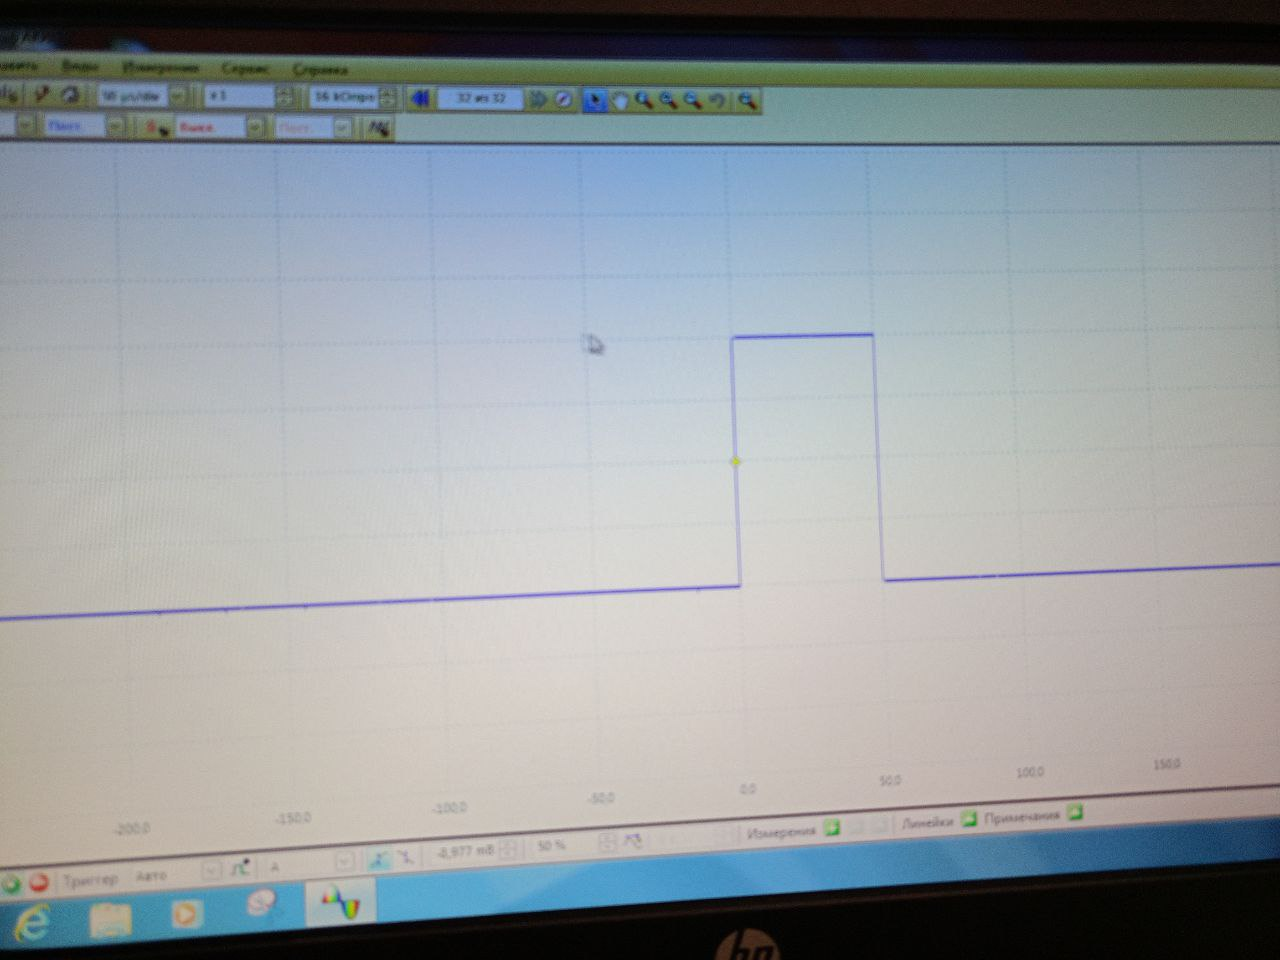
\includegraphics[width=.5\textwidth]{A.6.1.graph}
    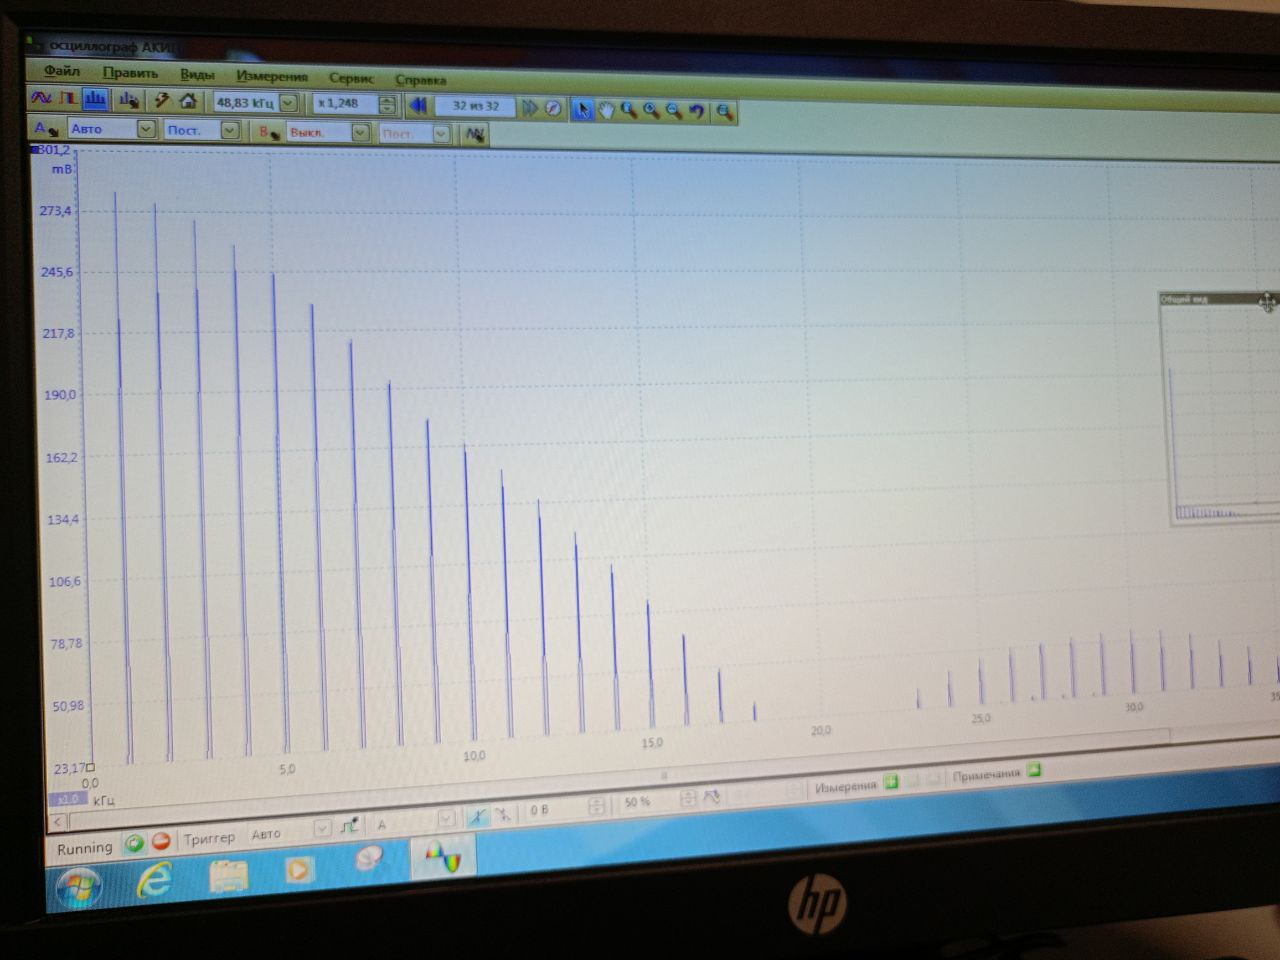
\includegraphics[width=.5\textwidth]{A.6.1.spectr}
    \caption{Сигнал и его спектр при параметрах, указанных выше}\label{fig:foobar}
\end{figure}

Теперь изменим по очереди каждый из указанных параметром и рассмотрим поведение сигнала и спектра

\begin{figure}[H]
    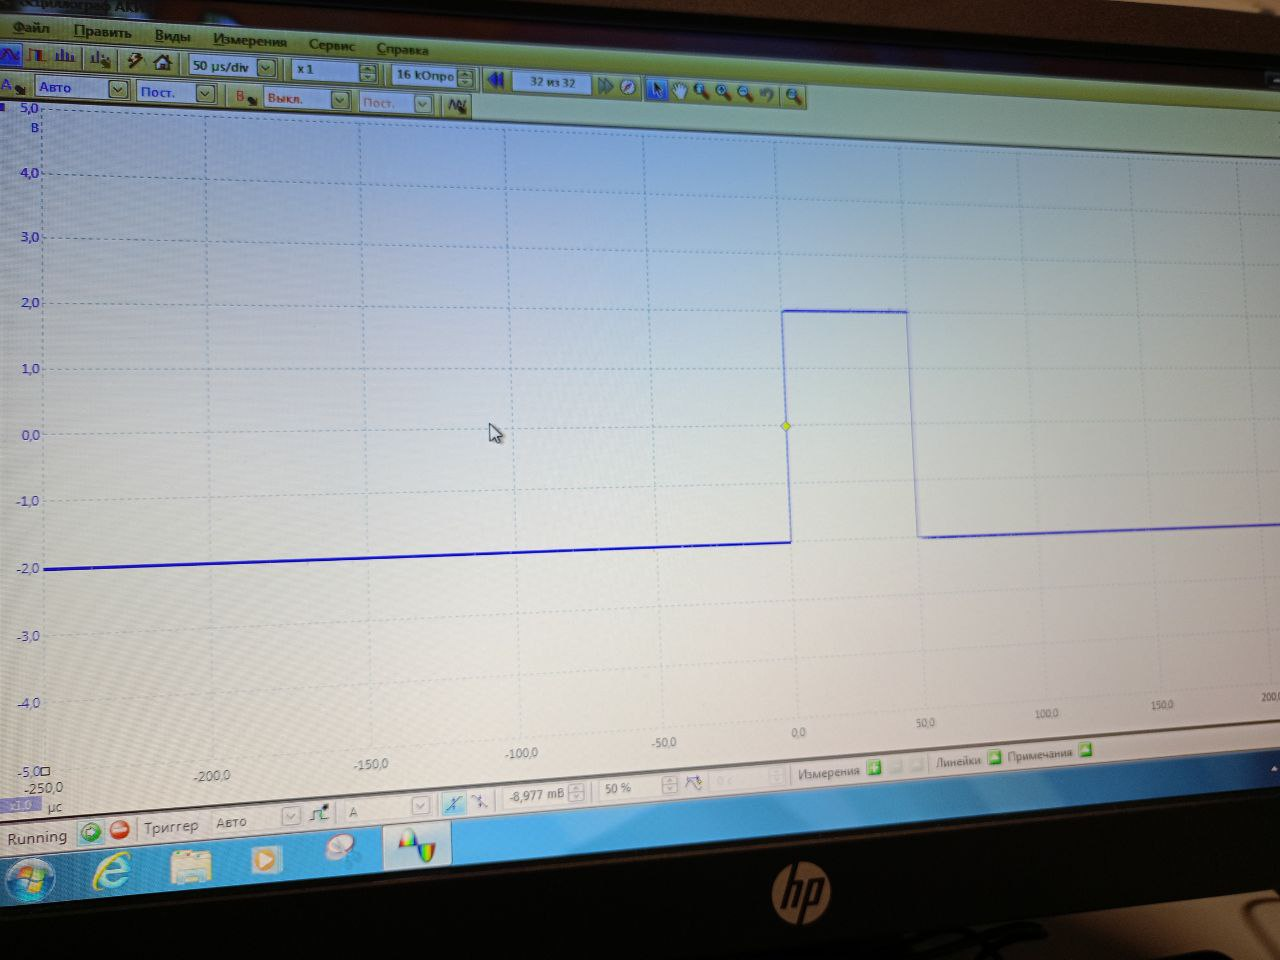
\includegraphics[width=.5\textwidth]{A.6.2.graph}
    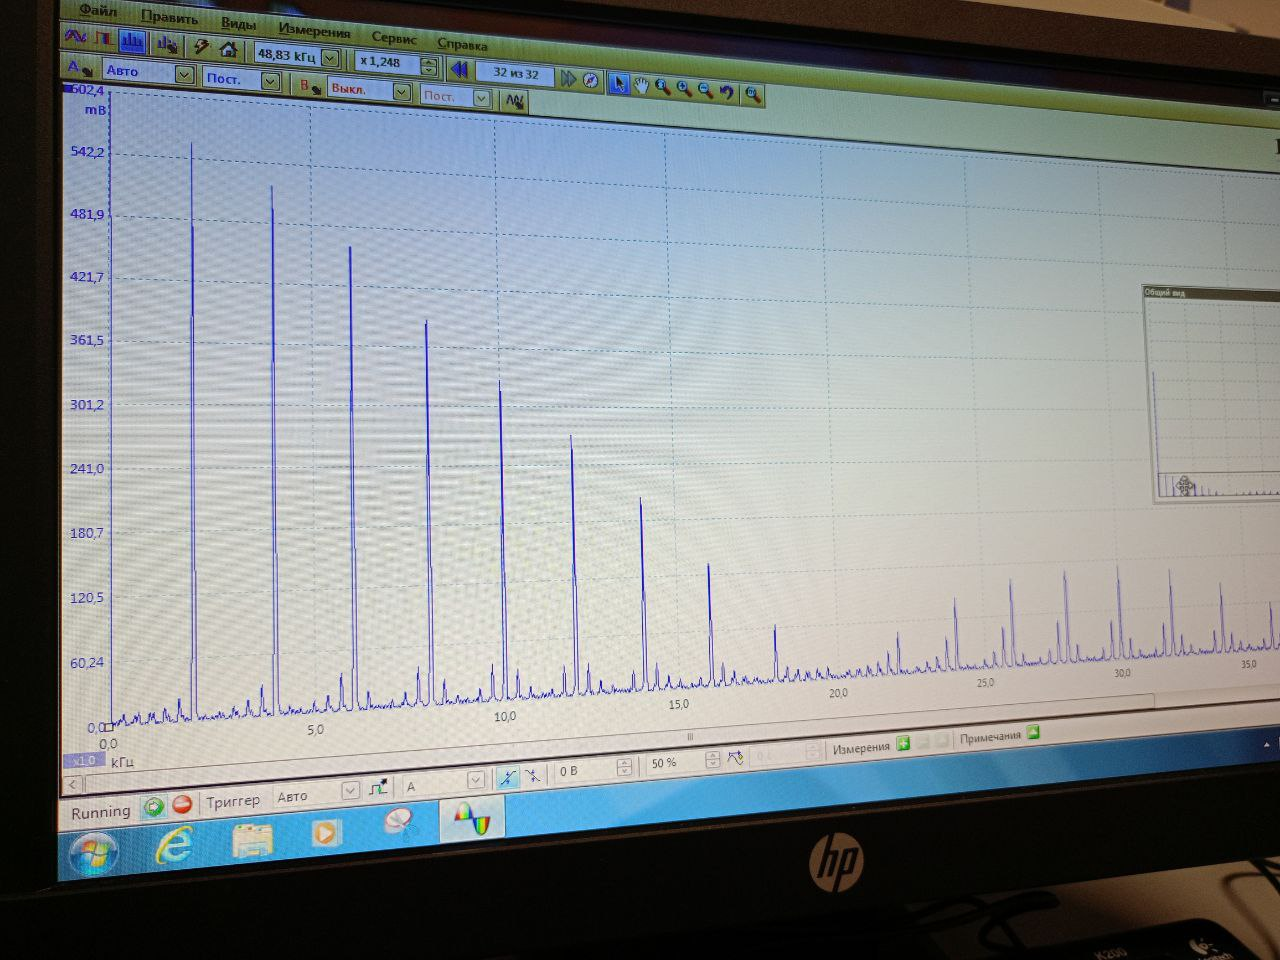
\includegraphics[width=.5\textwidth]{A.6.2.spectr}
    \caption{Сигнал и его спектр при $\nu_{\text{повт}} = 2 \text{кГц}, \tau = 50 \text{мкс}.$}\label{fig:foobar}
\end{figure}

\begin{figure}[H]
    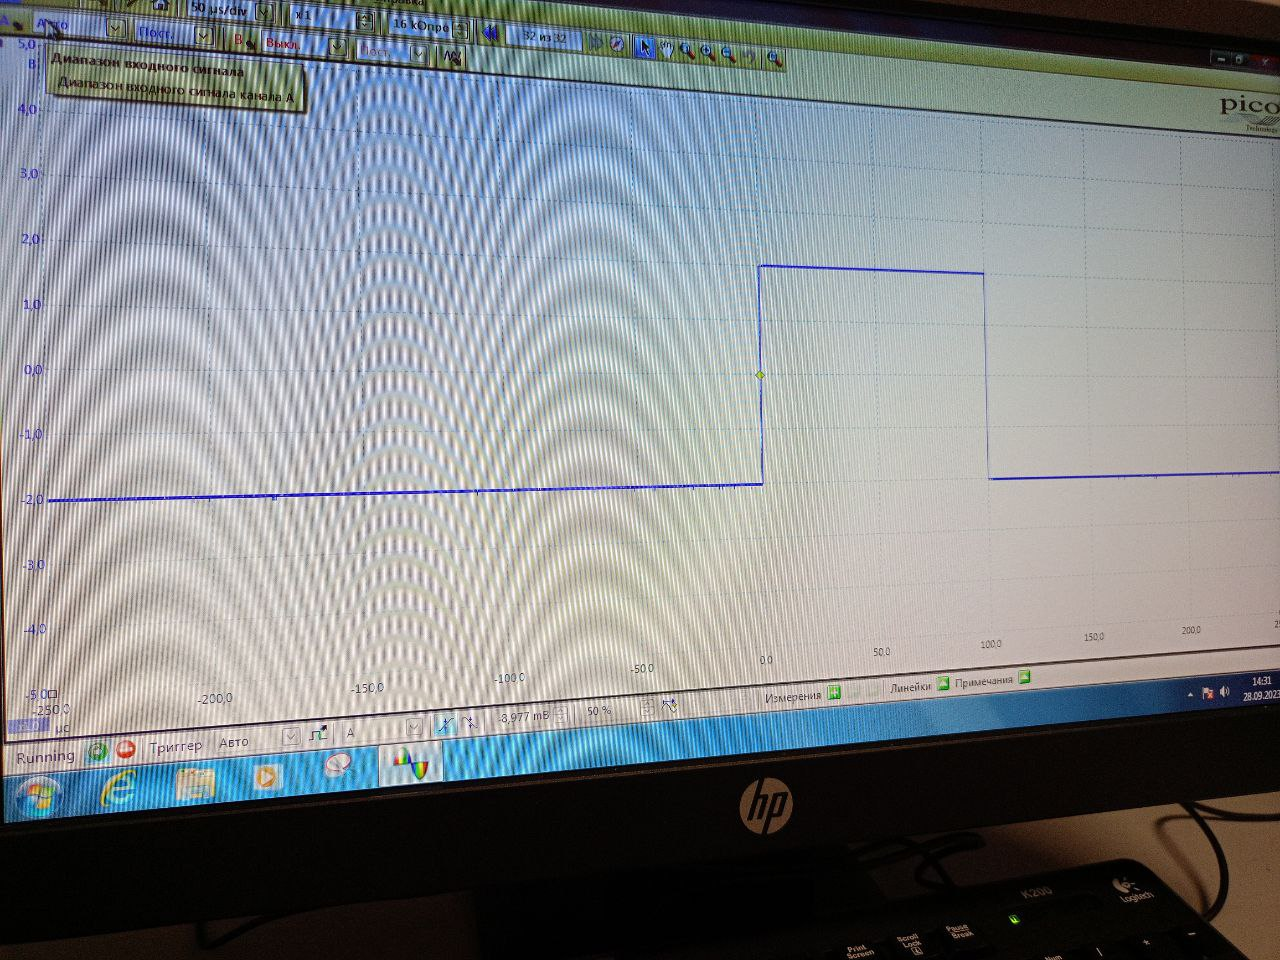
\includegraphics[width=.5\textwidth]{A.6.3.graph}
    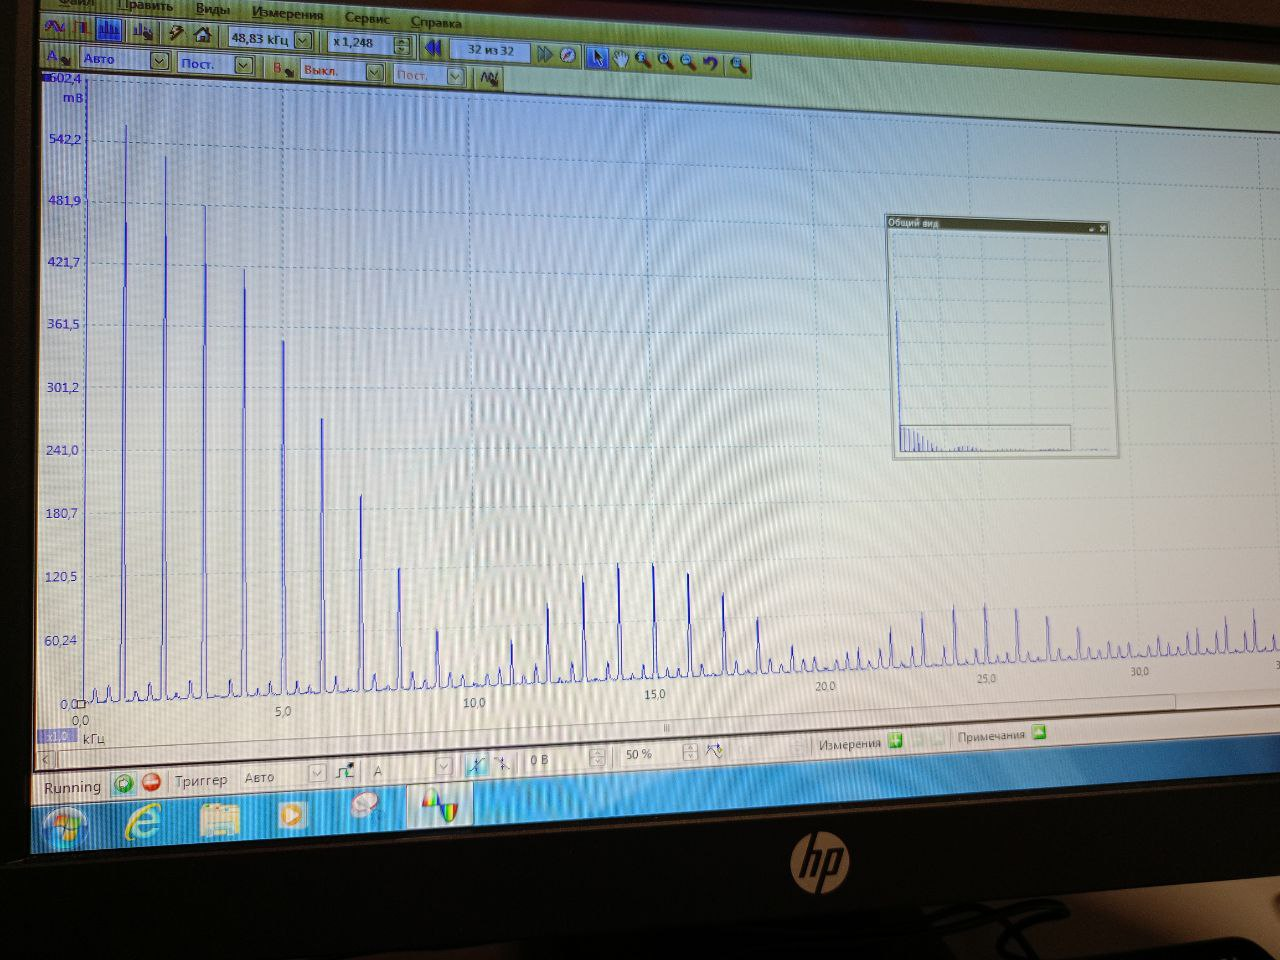
\includegraphics[width=.5\textwidth]{A.6.3.spectr}
    \caption{Сигнал и его спектр при $\nu_{\text{повт}} = 1 \text{кГц}, \tau = 100 \text{мкс}.$}\label{fig:foobar}
\end{figure}

\begin{figure}[H]
    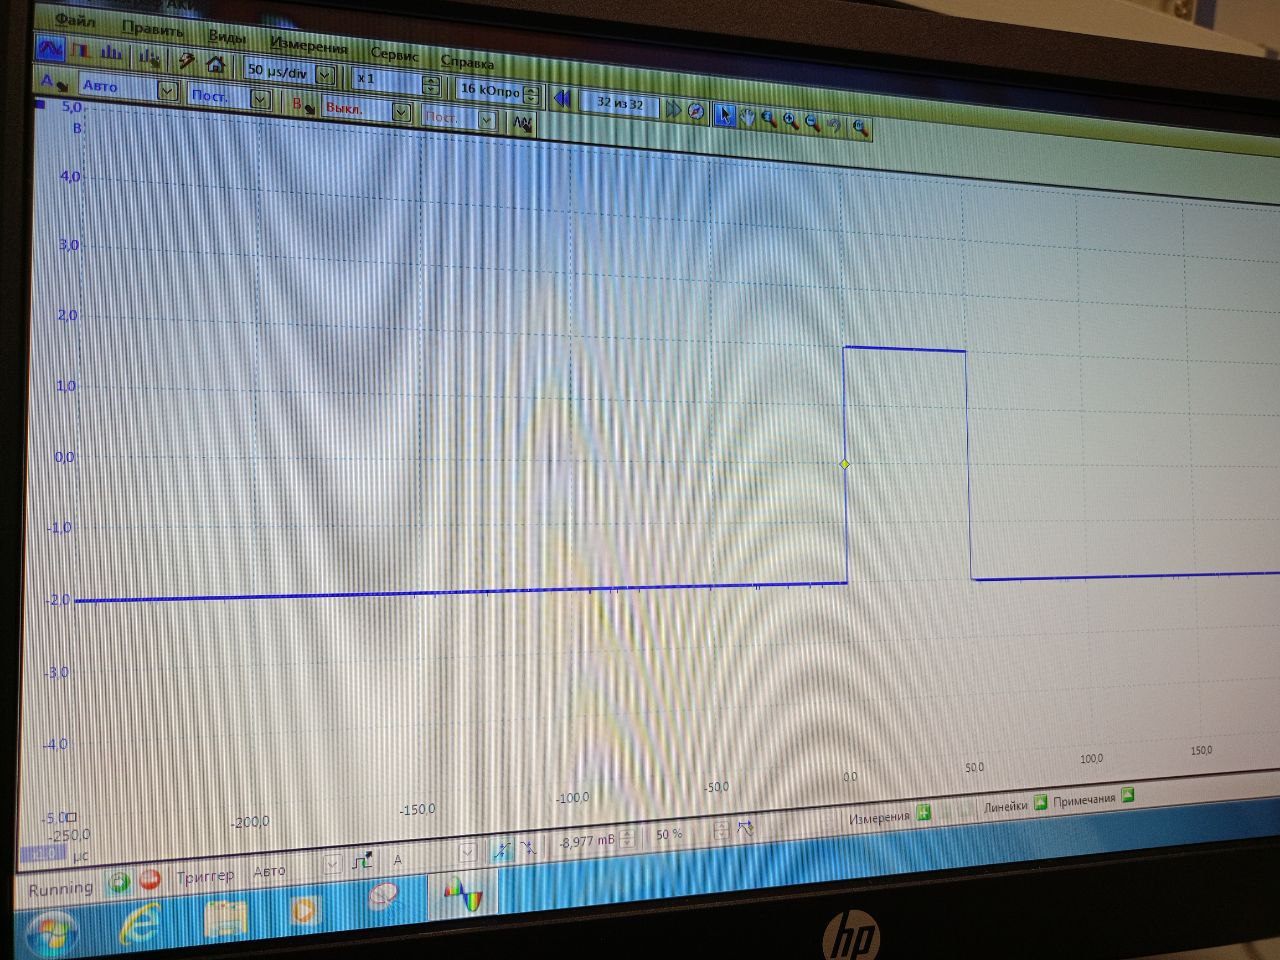
\includegraphics[width=.5\textwidth]{A.6.4.graph}
    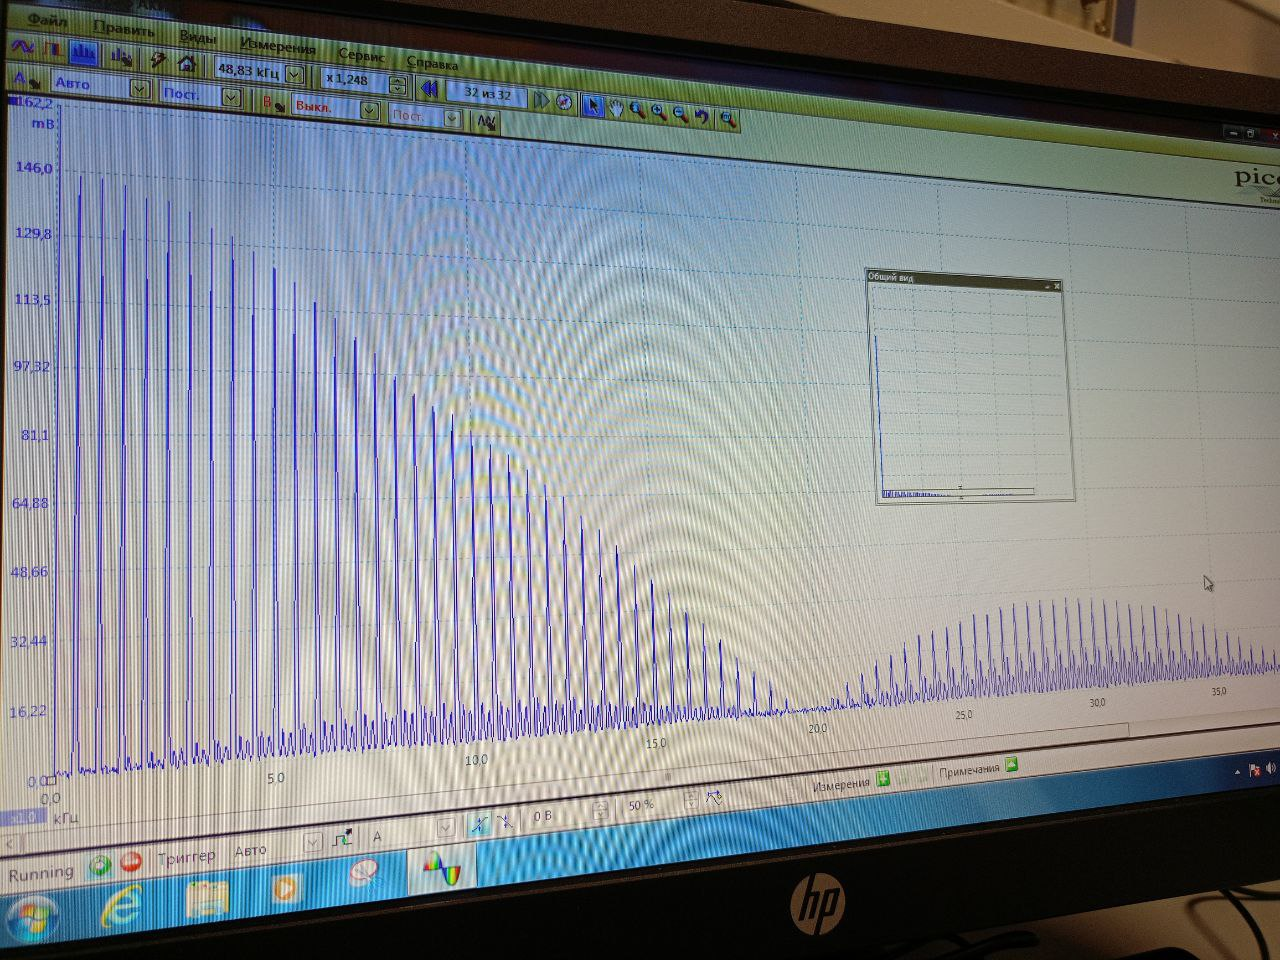
\includegraphics[width=.5\textwidth]{A.6.4.spectr}
    \caption{Сигнал и его спектр при $\nu_{\text{повт}} = 0,5 \text{кГц}, \tau = 500 \text{мкс}.$}\label{fig:foobar}
\end{figure}

Теперь измерим величины амплитуд и частот спектральных гармоник и сравним их с теоретическими. Начальные параметры изображены на картинке. 
\begin{figure}[H]
	\begin{center}	
    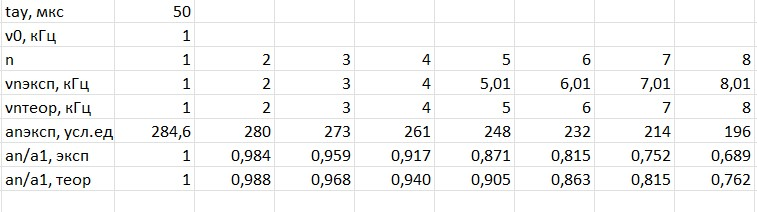
\includegraphics[width=.8\textwidth]{A.7.data}
    \end{center}
\end{figure}

Далее зафиксируем период повторения $T$ прямоугольного сигнала(начальные параметры T = 1мс) и будем менять длительность импульса $\tau$. Получим полную ширину спектра сигнала $\Delta \nu$, значение которой занесем в таблицу и по этим данным построим график зависимости $\Delta \nu(\frac{1}{\tau}$.

\begin{figure}[H]
	\begin{center}
    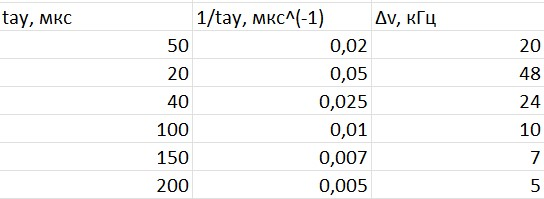
\includegraphics[width=.5\textwidth]{A.8.tabl}
\label{fig:foobar}
	\end{center}
\end{figure}

\begin{figure}[H]
	\begin{center}
    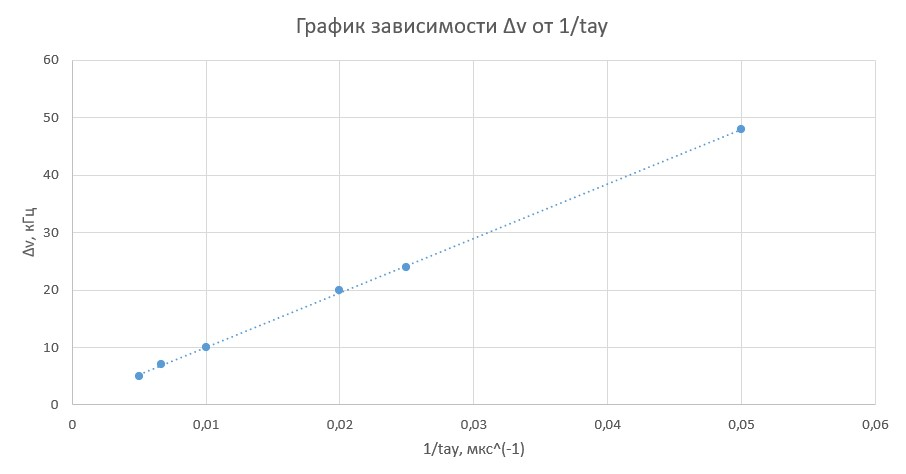
\includegraphics[width=.8\textwidth]{A.8.graph}
\label{fig:foobar}
	\end{center}
\end{figure}

Теперь же фиксируя длительность импульса прямоугольного сигнала($\tau = 100$ мкс) и изменяя период повторения T, измерим расстояния $\delta \nu = \nu_{n+1} - \nu_n$ между соседними гармониками спектра. Эти значения также занесем в таблицу и построим график зависимости $\delta \nu(\frac{1}{T})$.


\begin{figure}[H]
	\begin{center}
    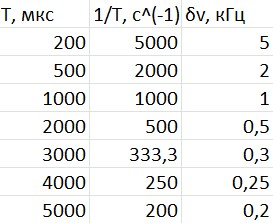
\includegraphics[width=.3\textwidth]{A.9.tabl}
\label{fig:foobar}
	\end{center}
\end{figure}

\begin{figure}[H]
	\begin{center}
    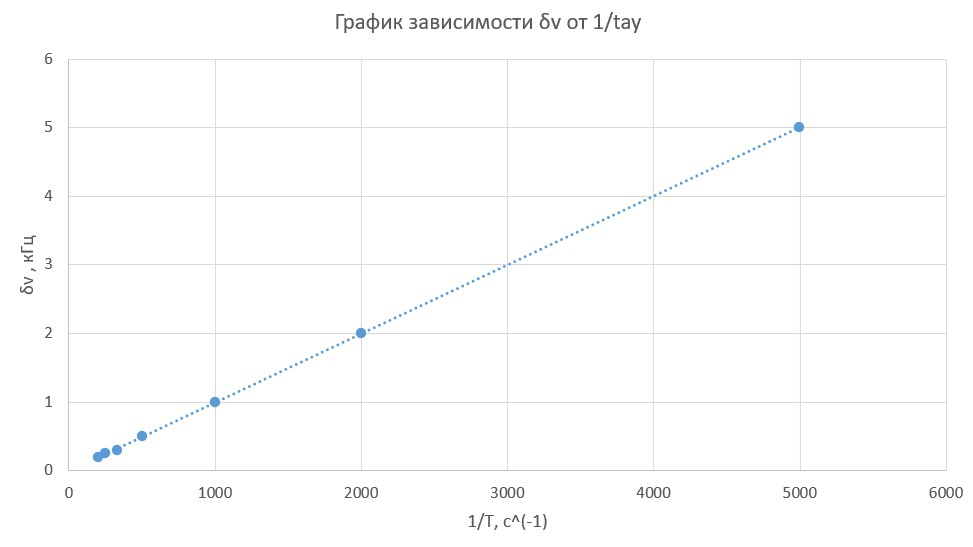
\includegraphics[width=.8\textwidth]{A.9.graph}
\label{fig:foobar}
	\end{center}
\end{figure}

Коэффициент наклона у первой прямой равен $k_1 = 0,95$, у второй же $k_2 = 1,002$. Оба этих значения лежат очень близко к числу 1, а это значит, что соотношение неопределенности выполняется(в обоих случаях характерное время получилось обратно пропорционально с коэффициентом 1 характерному масштабу).

\subsection*{Наблюдение спектра периодической последовательности цугов}

Теперь будем передавать периодические импульсы синусоидальной формы. Сначала подадим импульс при рекомендованных параметрах, а затем изменим каждый из параметров по очереди, чтобы исследовать как зависит спектр от данных величин. Рекомендуемые параметры $\nu_0 =$ 50 кГц, T = 1 мс,($\nu_{\text{повт}} = $ 1 кГц), N = 5(число периодов в синусоиде одного импульса), $\tau = \frac{N}{\nu_0} = $ 100 мкс.
\newpage
\begin{figure}[H]
\begin{center}
    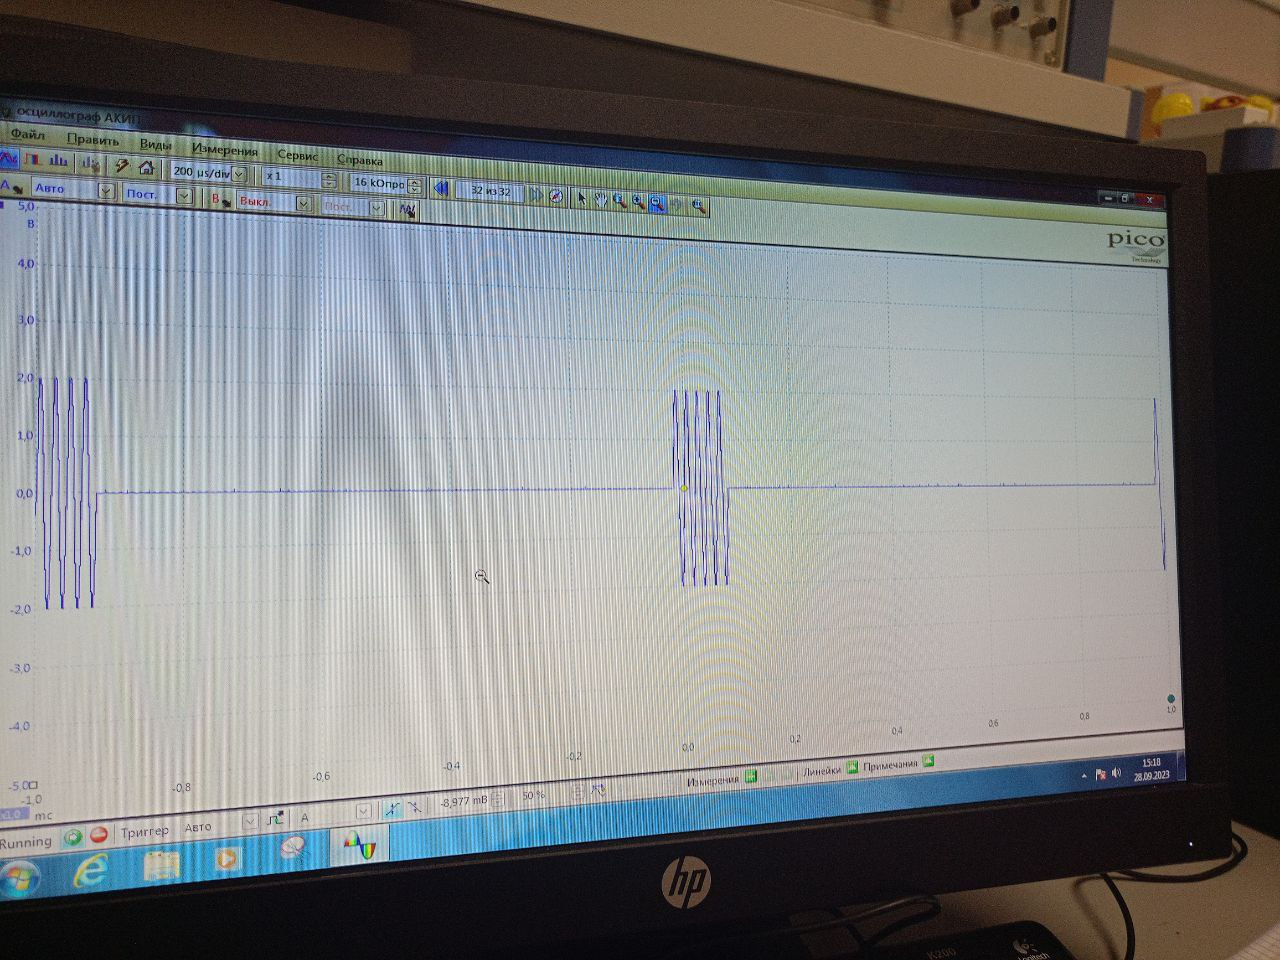
\includegraphics[width=.6\textwidth]{B.13.1.graph}
\end{center}
\end{figure}

\begin{figure}[H]
    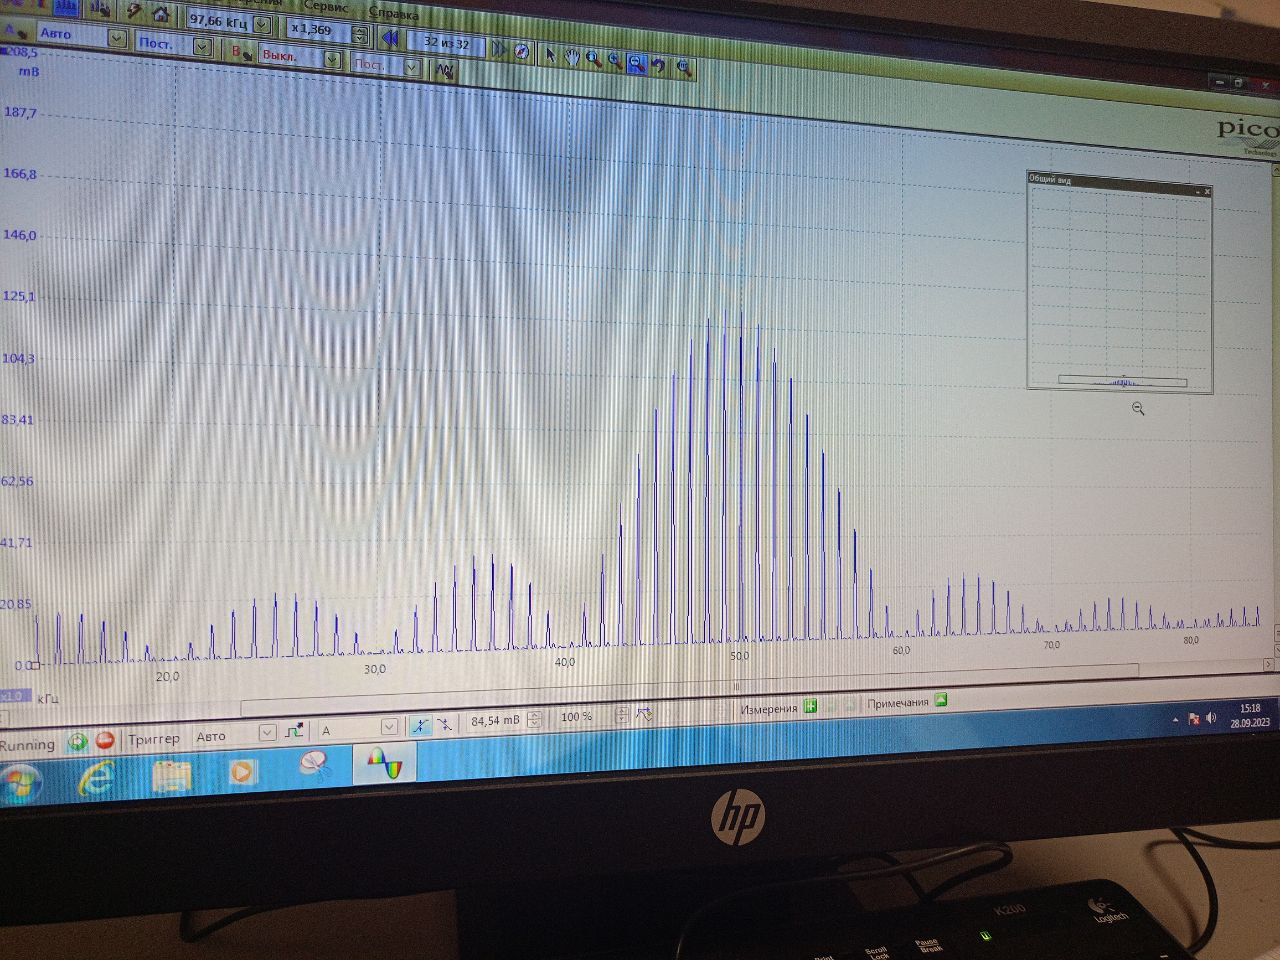
\includegraphics[width=.9\textwidth]{B.13.1.spectr}
    \caption{Сигнал и его спектр при параметрах, указанных выше}\label{fig:foobar}
\end{figure}


\begin{figure}[H]
\begin{center}
    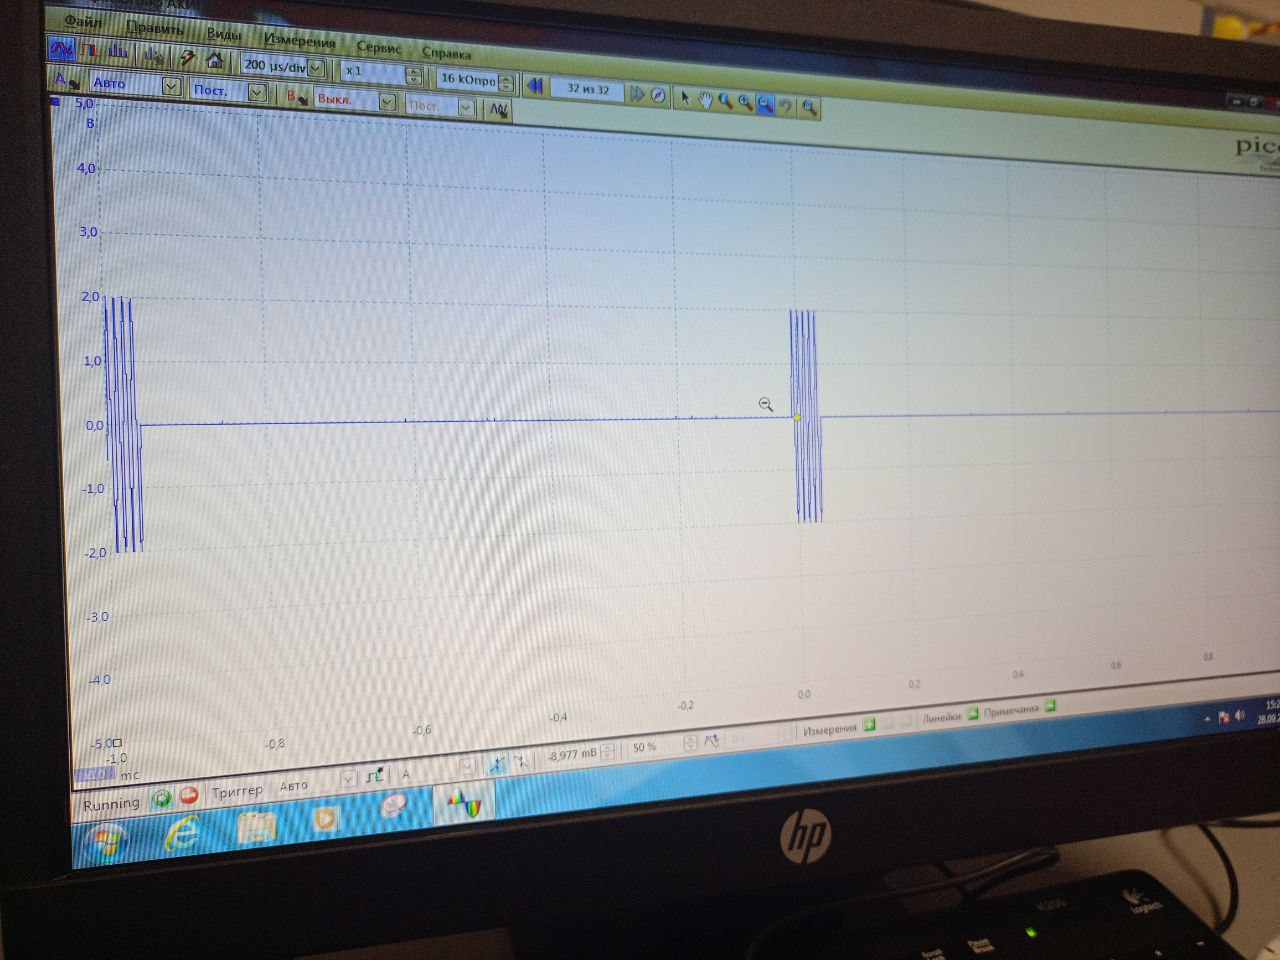
\includegraphics[width=.6\textwidth]{B.13.2.graph}
\end{center}
\end{figure}

\begin{figure}[H]
    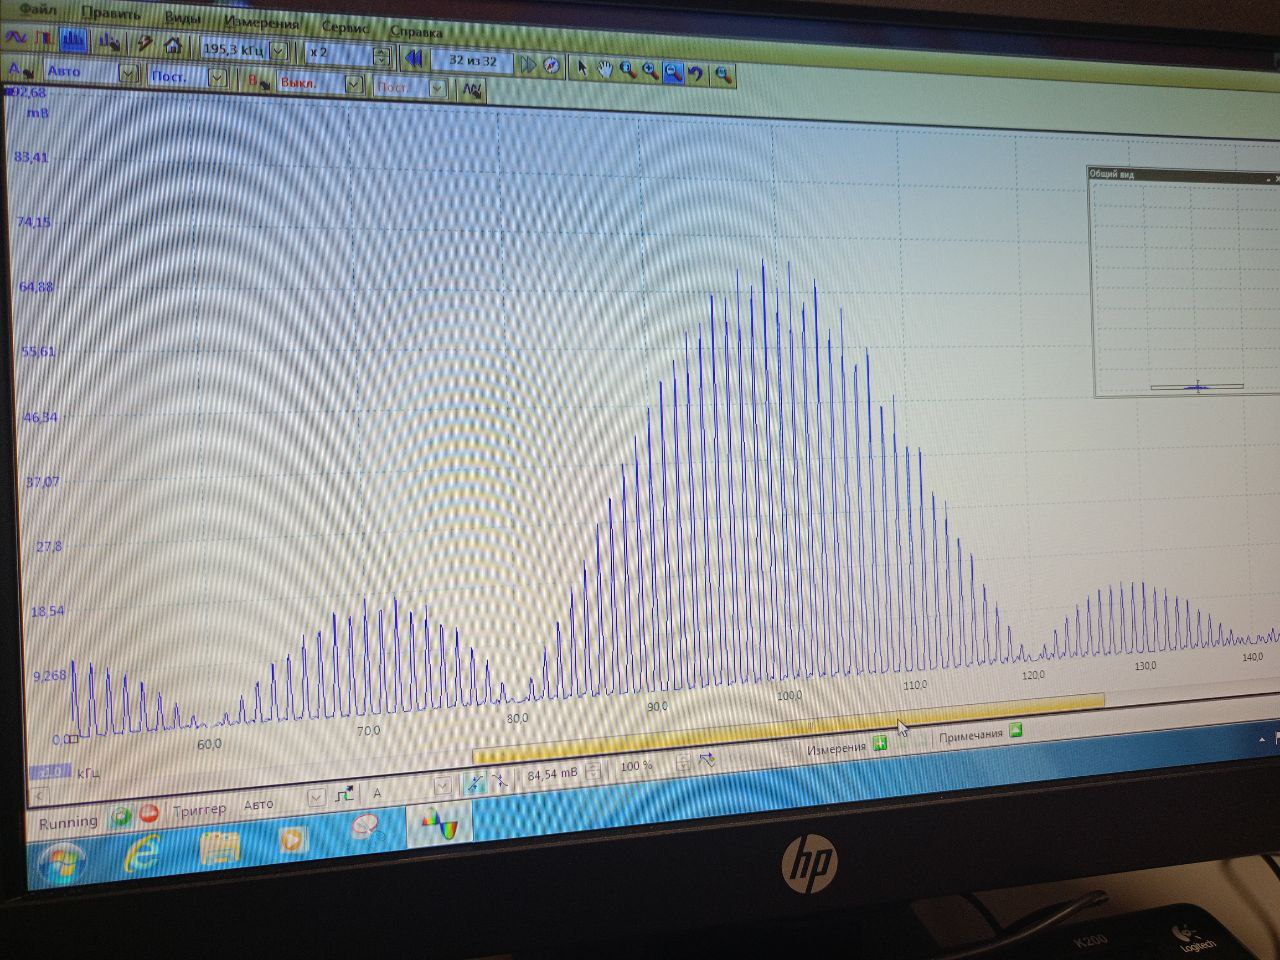
\includegraphics[width=.9\textwidth]{B.13.2.spectr}
    \caption{Сигнал и его спектр при $\nu_{0} = 100 \text{кГц}, T = 1 \text{мс}, N = 5.$}\label{fig:foobar}
\end{figure}

\begin{figure}[H]
\begin{center}
    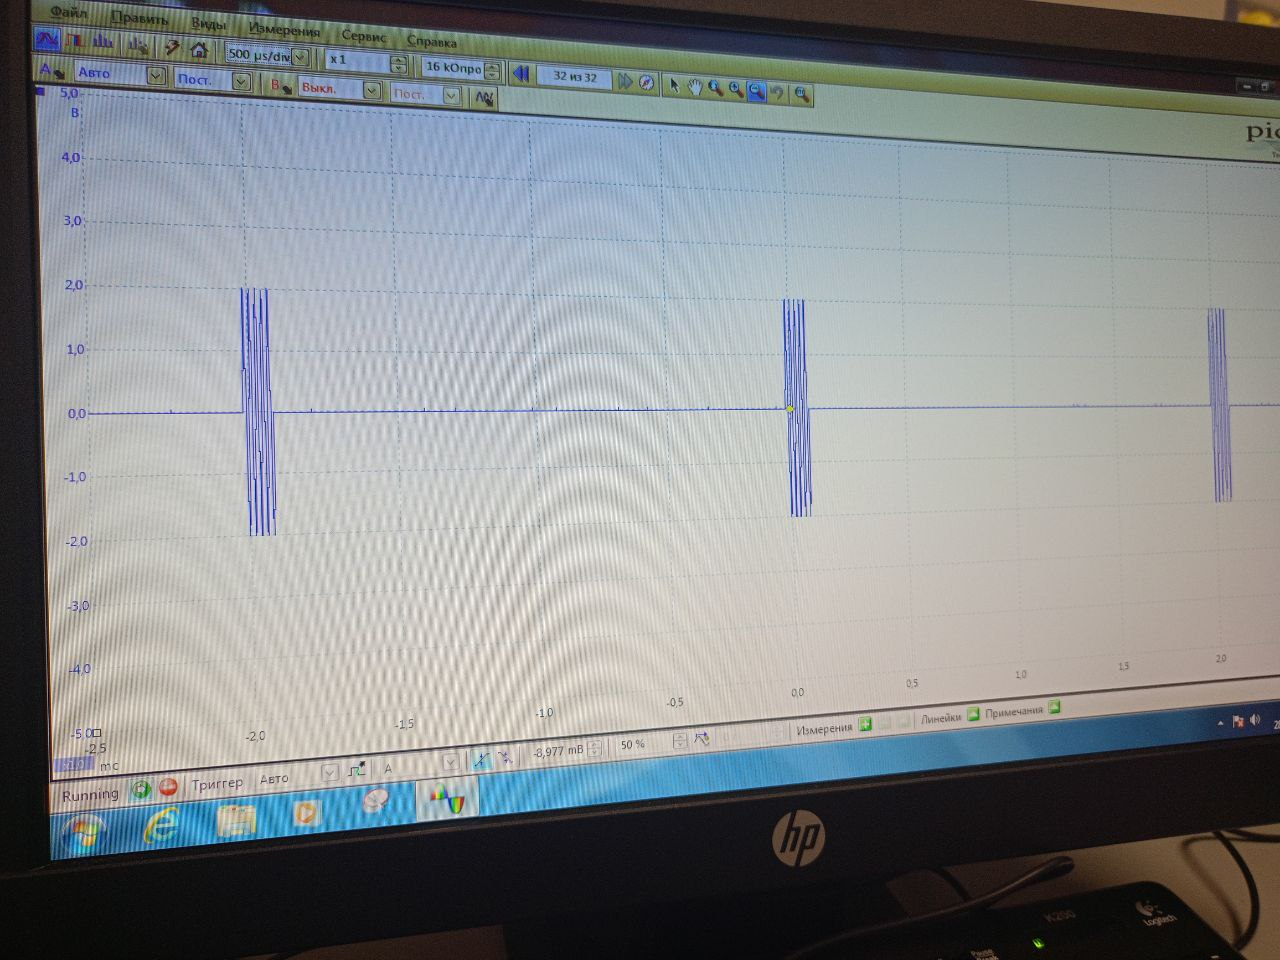
\includegraphics[width=.6\textwidth]{B.13.3.graph}
\end{center}
\end{figure}

\begin{figure}[H]
    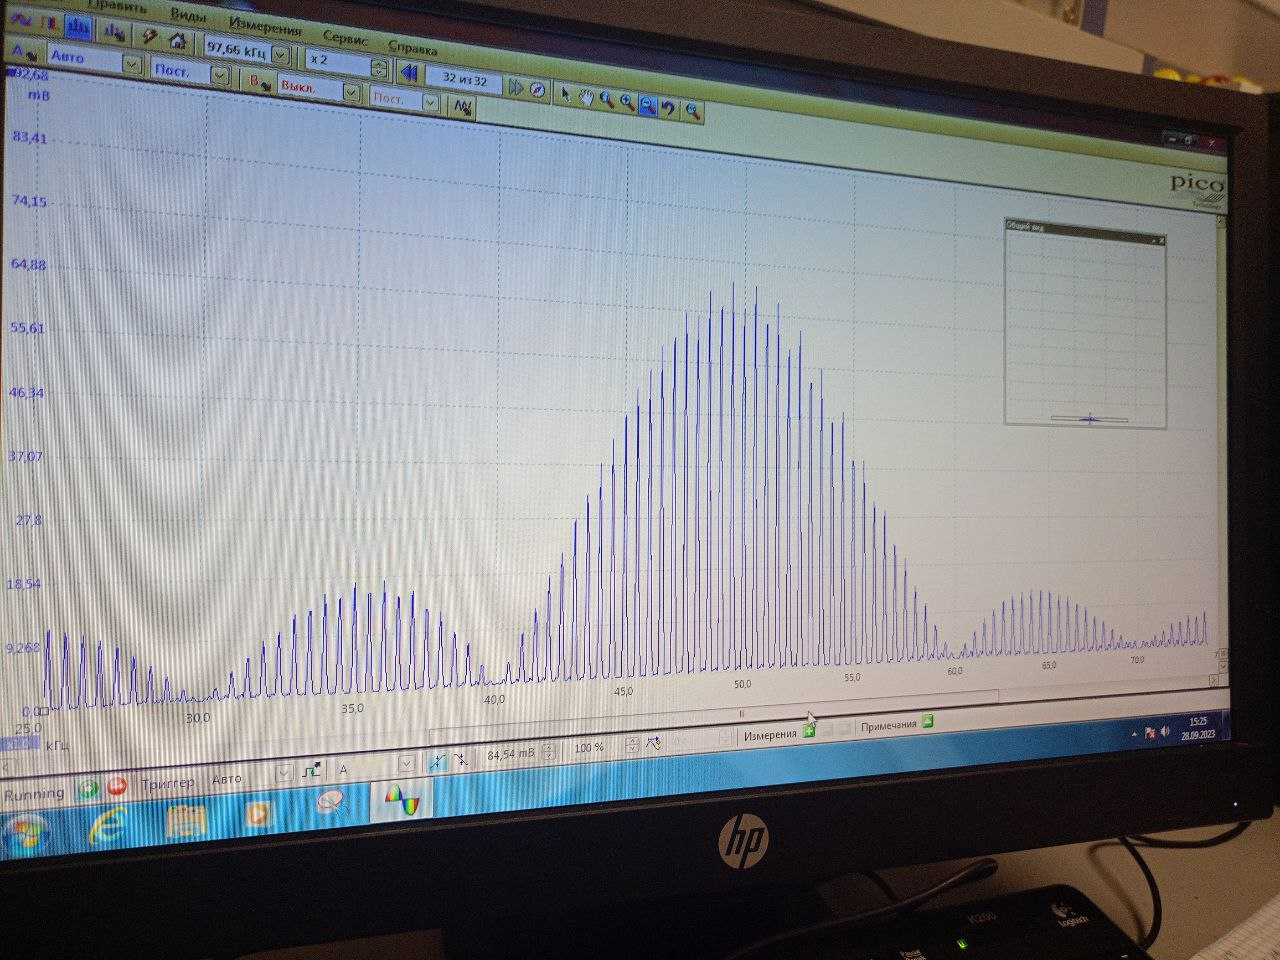
\includegraphics[width=.9\textwidth]{B.13.3.spectr}
    \caption{Сигнал и его спектр при $\nu_{0} = 50 \text{кГц}, T = 2 \text{мс}, N = 5.$}\label{fig:foobar}
\end{figure}

\begin{figure}[H]
\begin{center}
    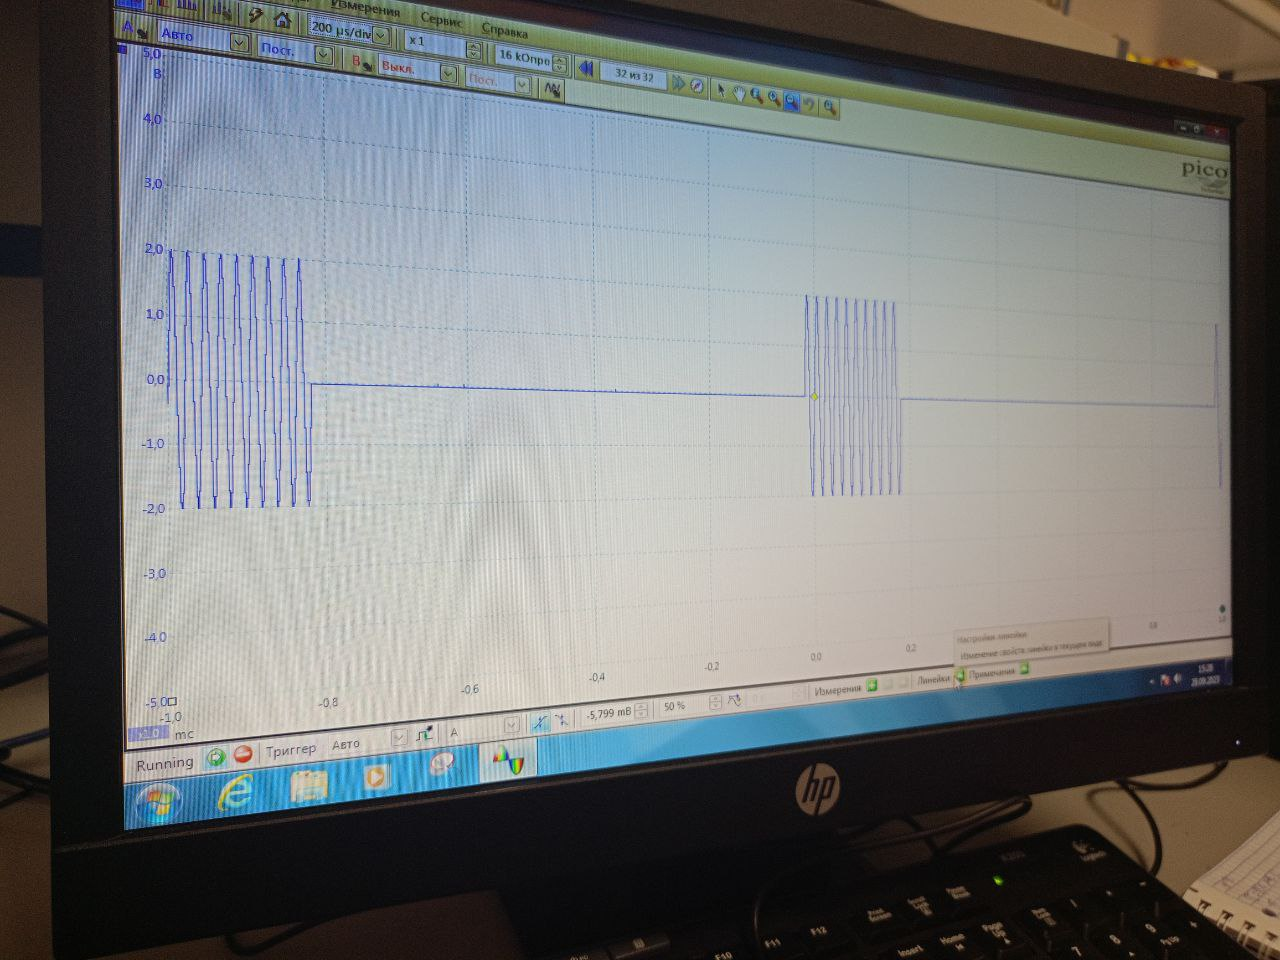
\includegraphics[width=.6\textwidth]{B.13.4.graph}
\end{center}
\end{figure}

\begin{figure}[H]
    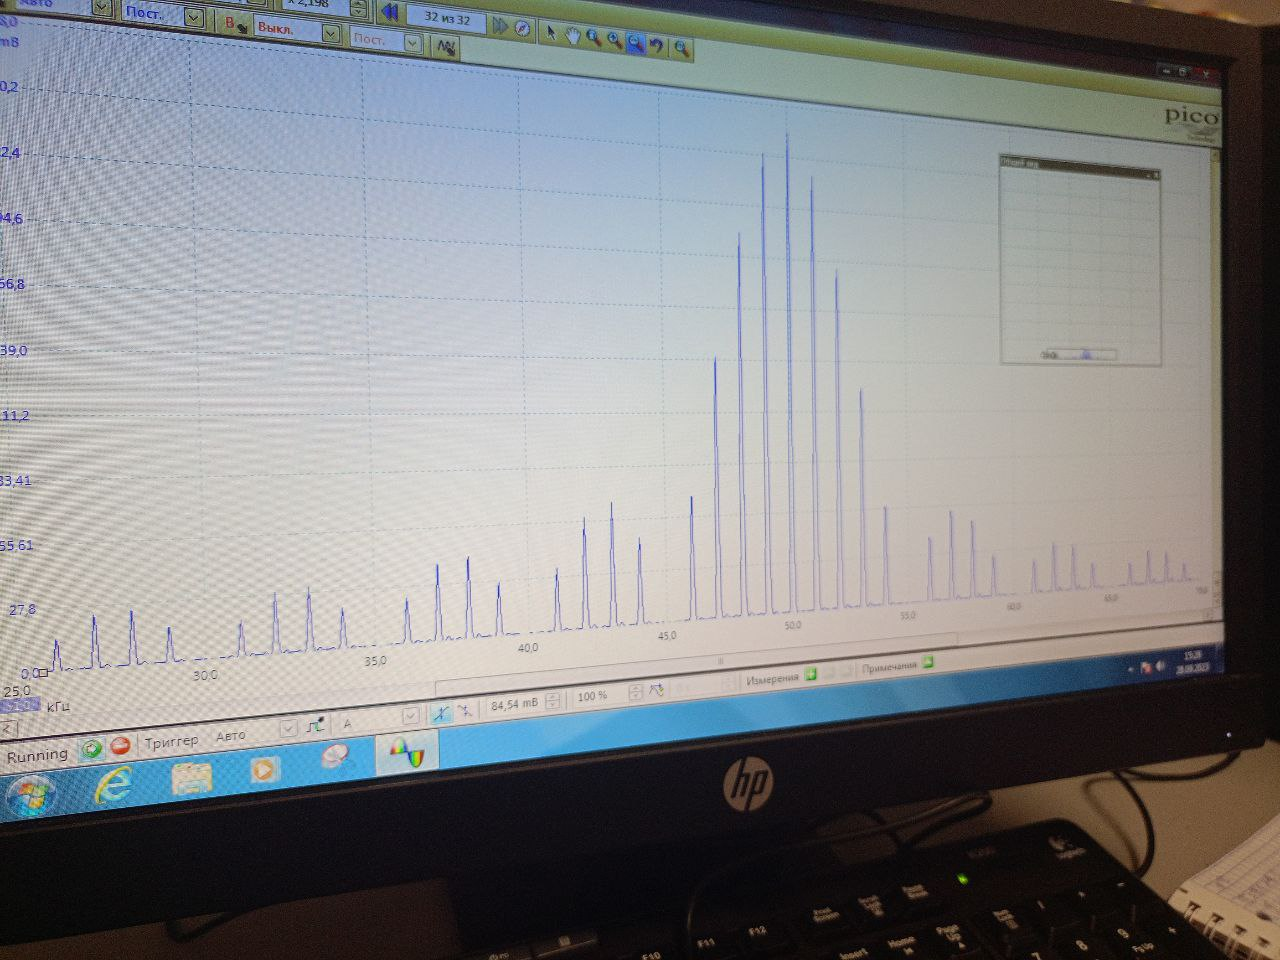
\includegraphics[width=.9\textwidth]{B.13.4.spectr}
    \caption{Сигнал и его спектр при $\nu_{0} = 50 \text{кГц}, T = 1 \text{мс}, N = 10.$}\label{fig:foobar}
\end{figure}

Теперь измерим при каждом из данных рассмотренных импульсах расстояние между гармониками спектра $\delta \nu$ и ширину спектра $\Delta \nu$. Построим таблицы и графики зависимостей $\delta \nu(\frac{1}{\tau})$ и $\Delta \nu (\frac{1}{T})$

\begin{figure}[H]
\begin{center}
    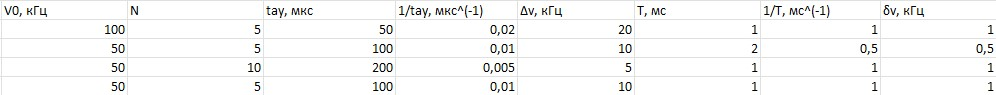
\includegraphics[width=1\textwidth]{B.15.tabl}
\end{center}
\end{figure}

\begin{figure}[H]
    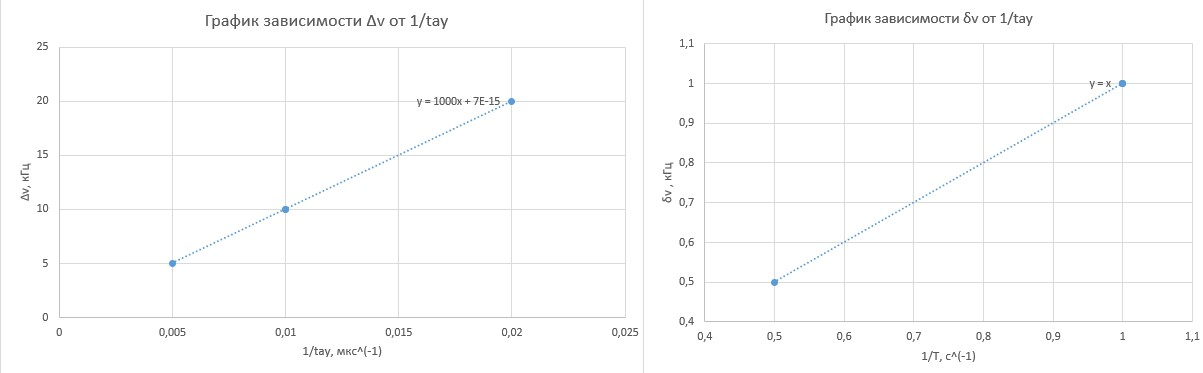
\includegraphics[width=1\textwidth]{B.15.grapg}
\end{figure}

Из графиков видно, что соотношения неопределенностей выполняются.

\subsection*{Исследование спектра амплитудно-модулированного сигнала}
Установим рекомендуемые параметры нашего сигнала. $\nu_0 = 50$ кГц, $\nu_{\text{мод}} = 2$ кГц, $m = 0,5(50\%)$.

Теперь измерим максимальную и минимальную амплитуды сигнала. Получается $A_{max} = 1,511 $ В, $A_{min} = 0,507$ В. Равенство $m = \frac{A_{max} - A_{min}}{A_{max} + A_{min}}$ выполняется.

Далее, изменяя частоты, рассмотрим изменение спектра сигнала.
\begin{figure}[H]
\begin{center}
    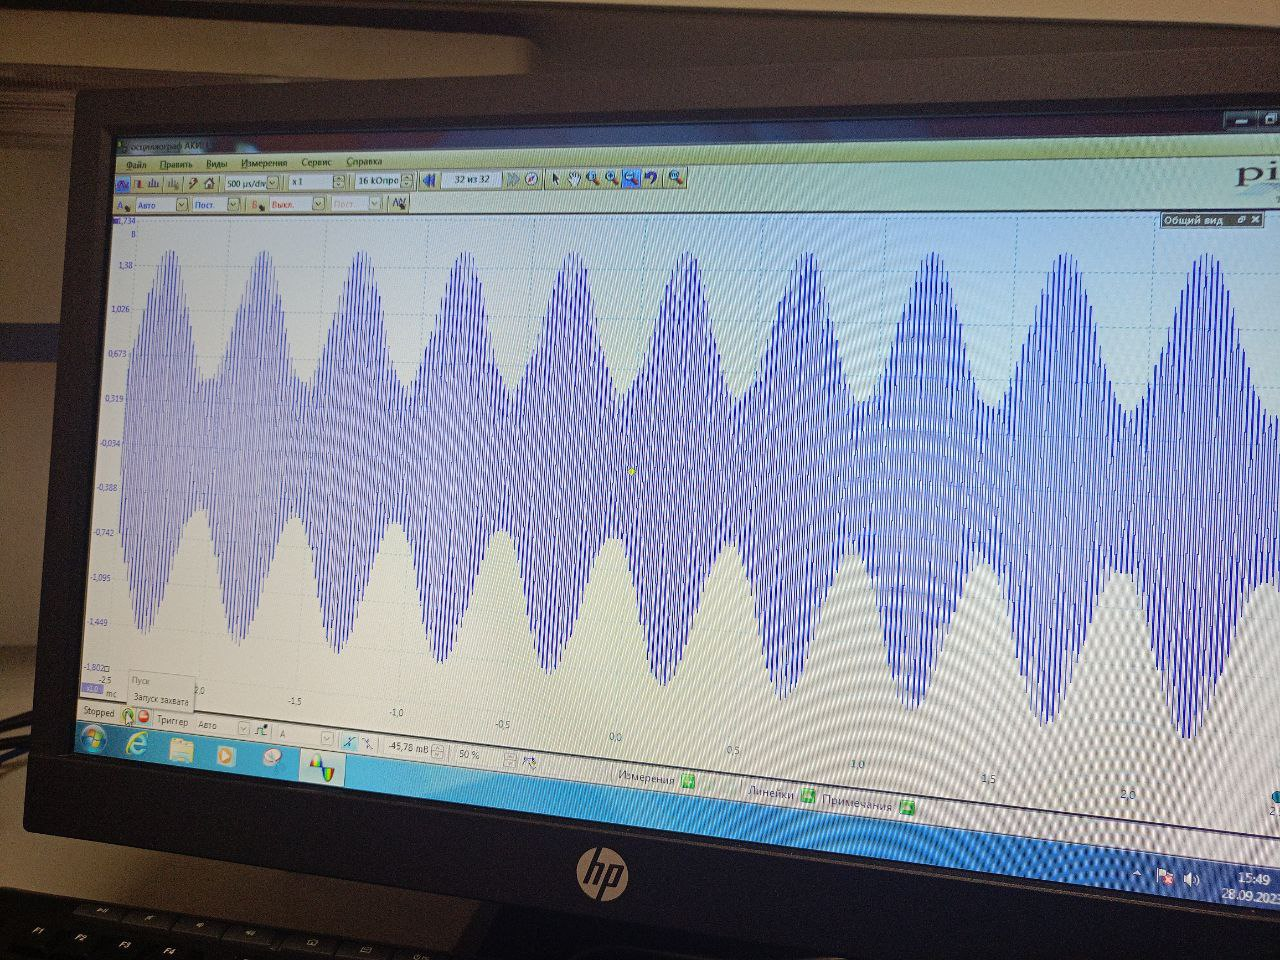
\includegraphics[width=.5\textwidth]{G.21.1.graph}
\end{center}
\end{figure}

\begin{figure}[H]
\begin{center}
    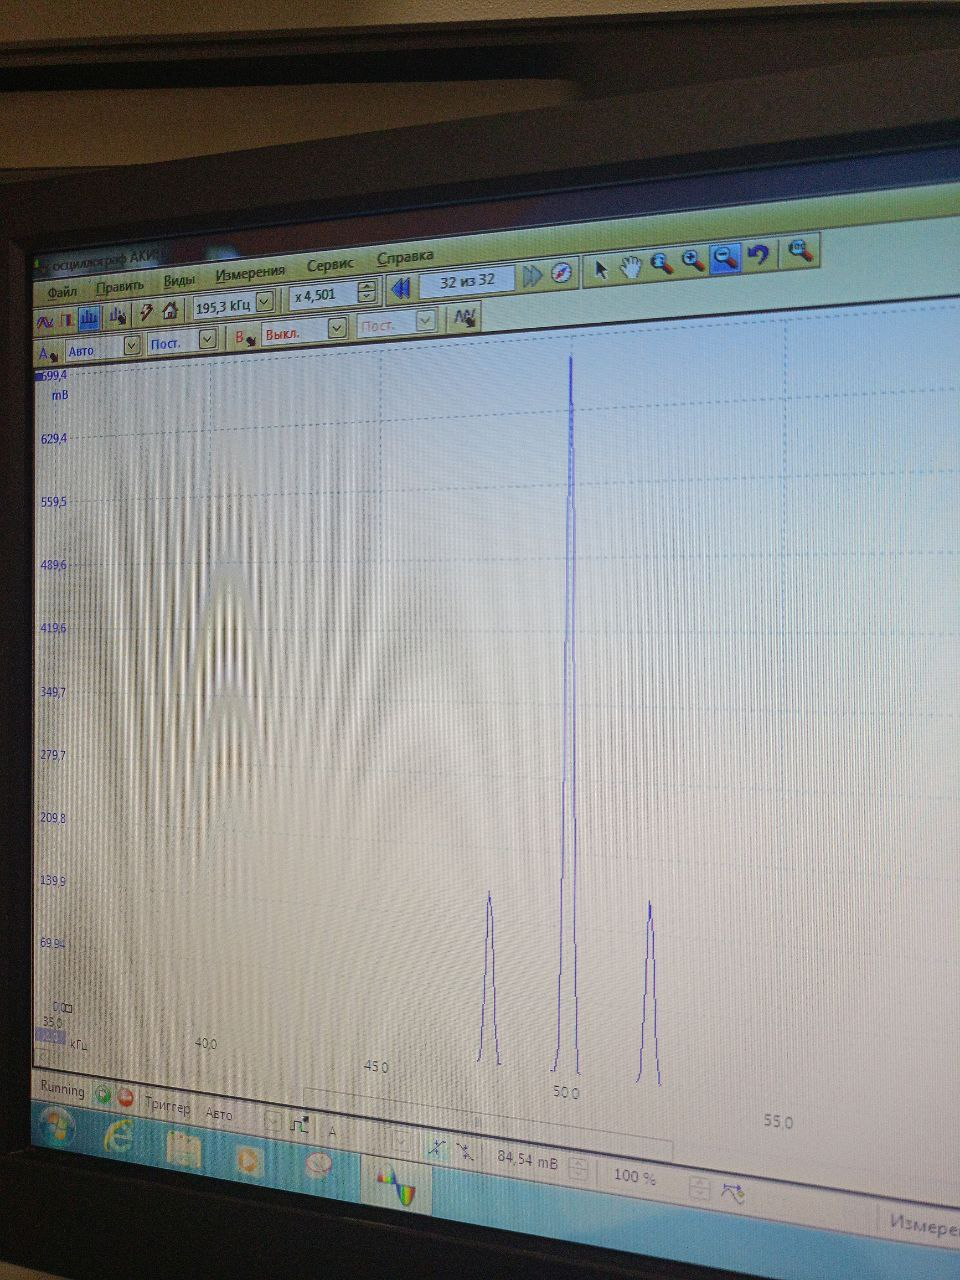
\includegraphics[width=.5\textwidth]{G.21.1.spectr}
    \caption{Сигнал и его спектр при параметрах, указанных выше}\label{fig:foobar}
\end{center}
\end{figure}


\begin{figure}[H]
\begin{center}
    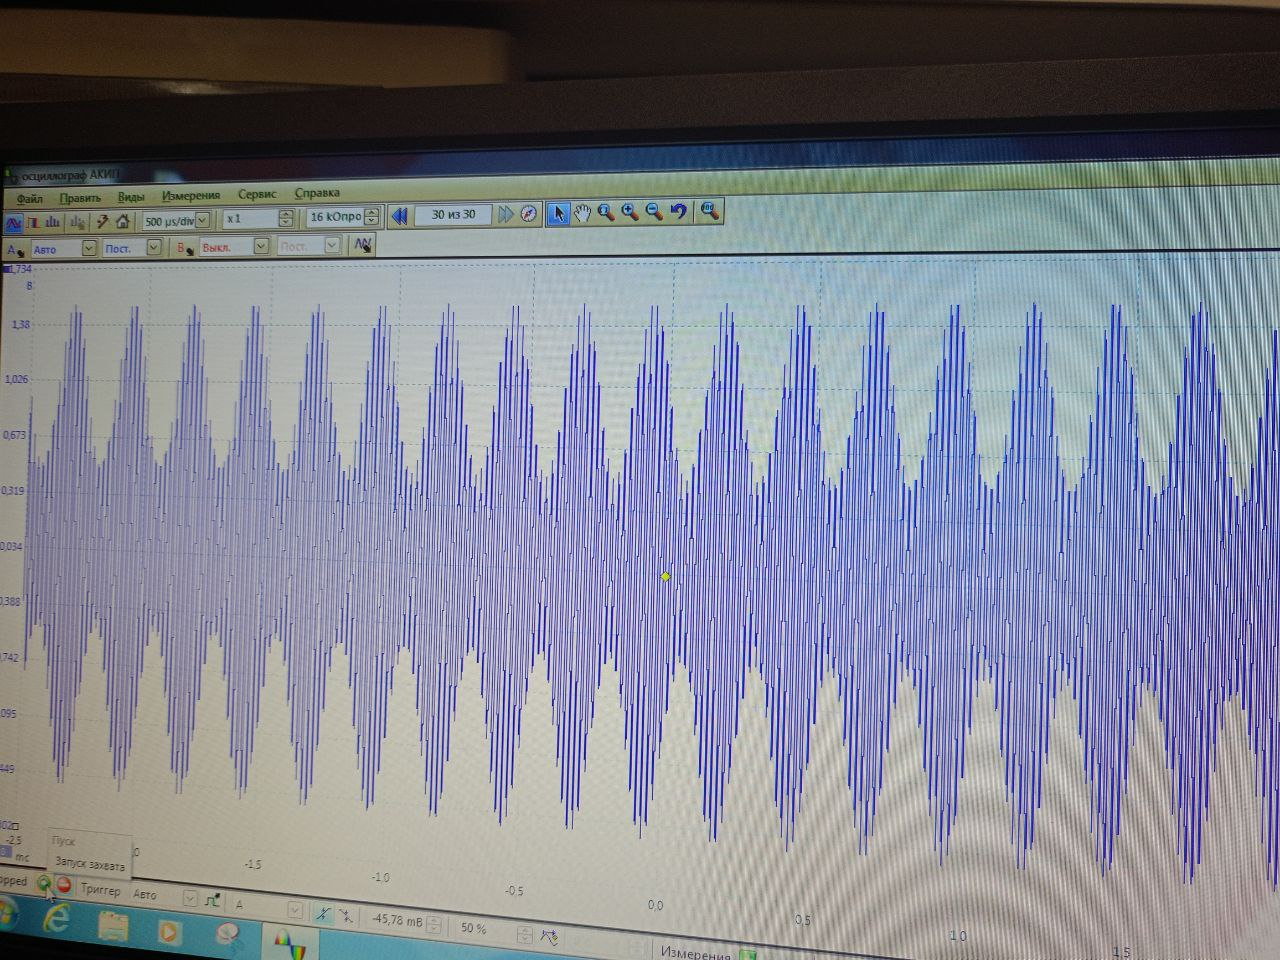
\includegraphics[width=.5\textwidth]{G.21.2.graph}
\end{center}
\end{figure}

\begin{figure}[H]
\begin{center}
    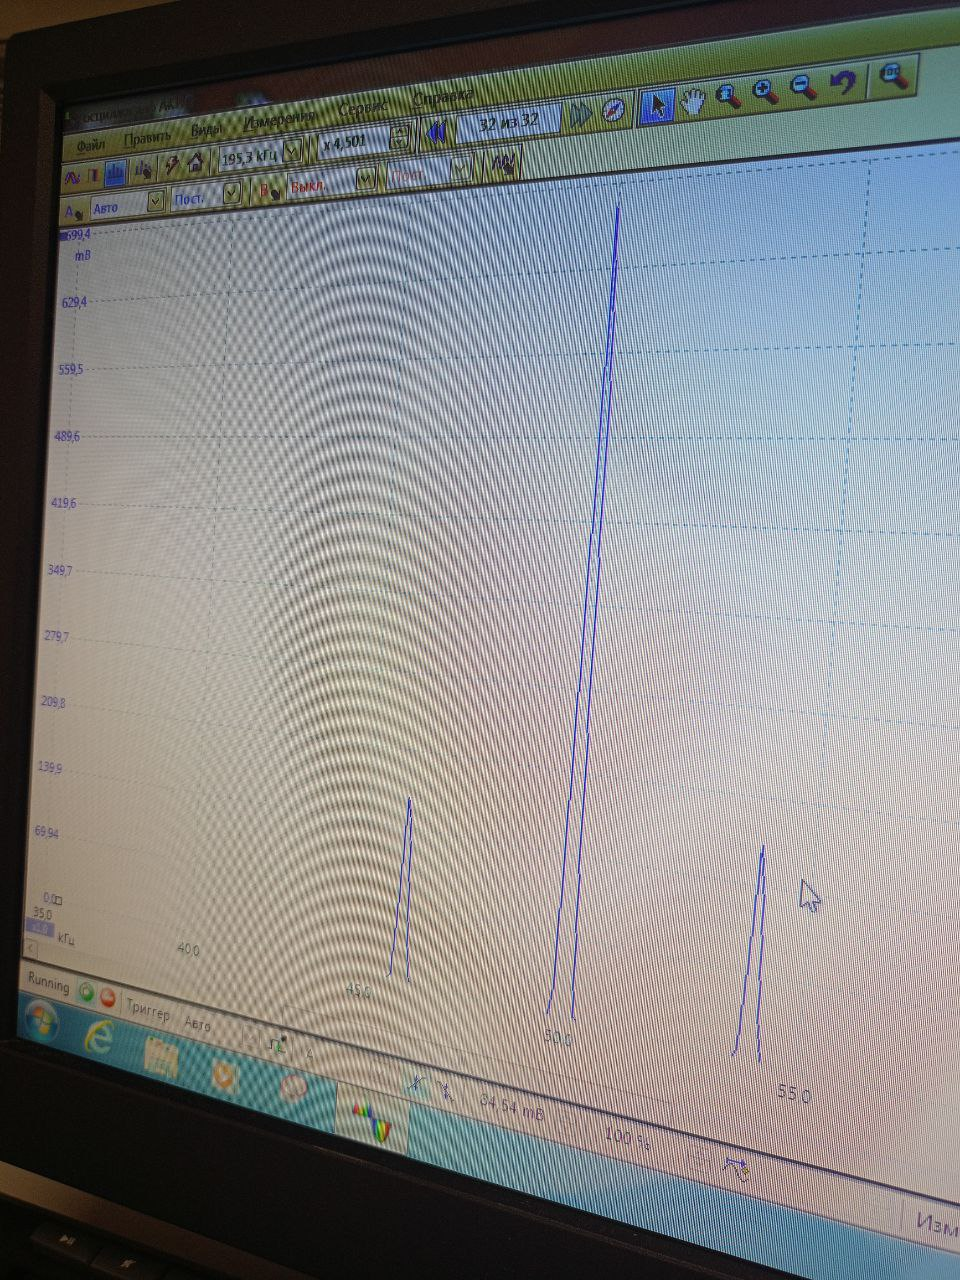
\includegraphics[width=.5\textwidth]{G.21.2.spectr}
    \caption{Сигнал и его спектр при $\nu_{\text{мод}} = 2 \text{кГц}, \nu_0 = 100 \text{кГц}.$}\label{fig:foobar}
\end{center}
\end{figure}

\begin{figure}[H]
\begin{center}
    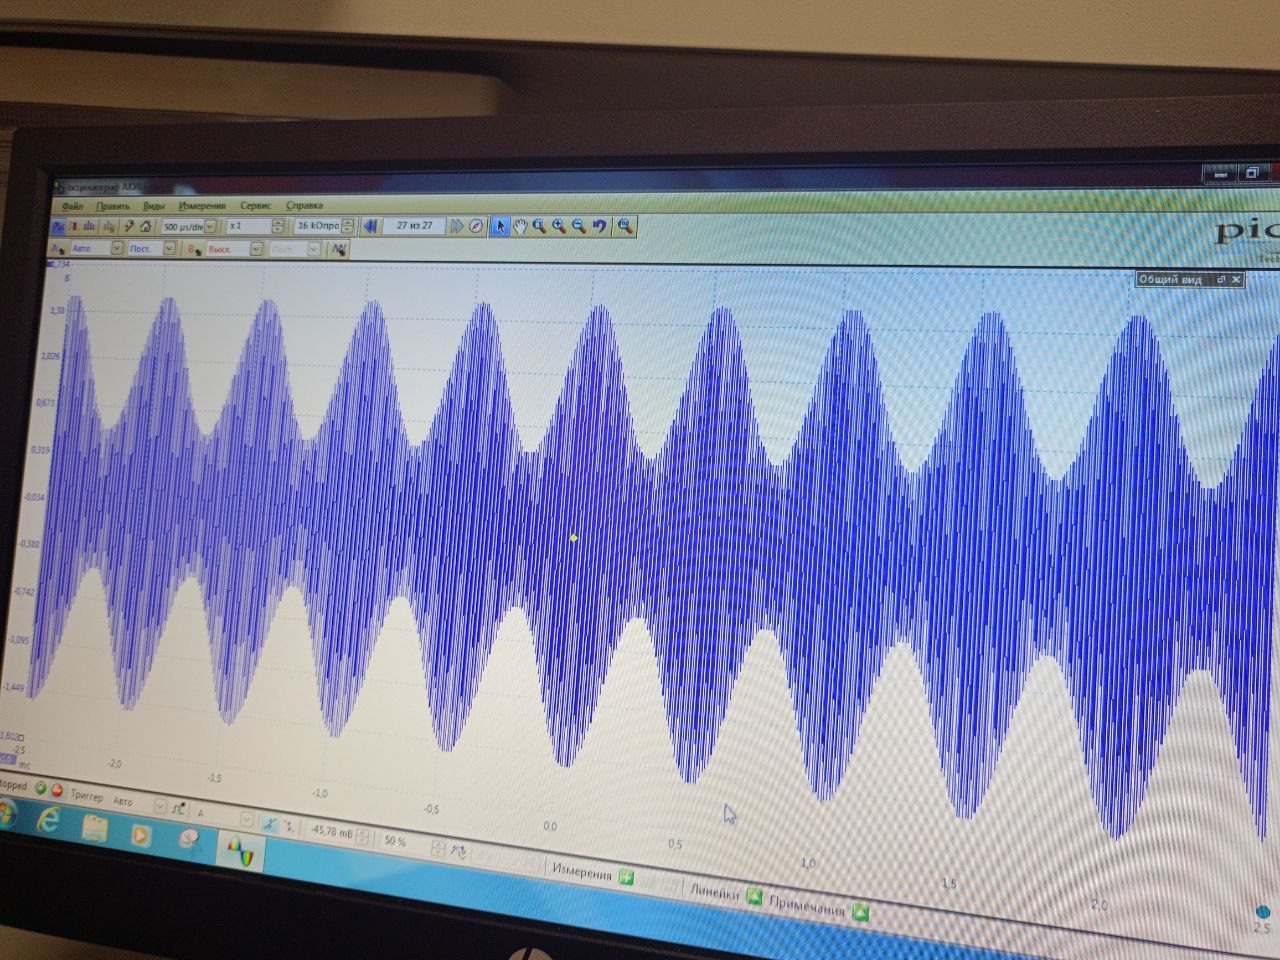
\includegraphics[width=.5\textwidth]{G.21.3.graph}
\end{center}
\end{figure}

\begin{figure}[H]
\begin{center}
    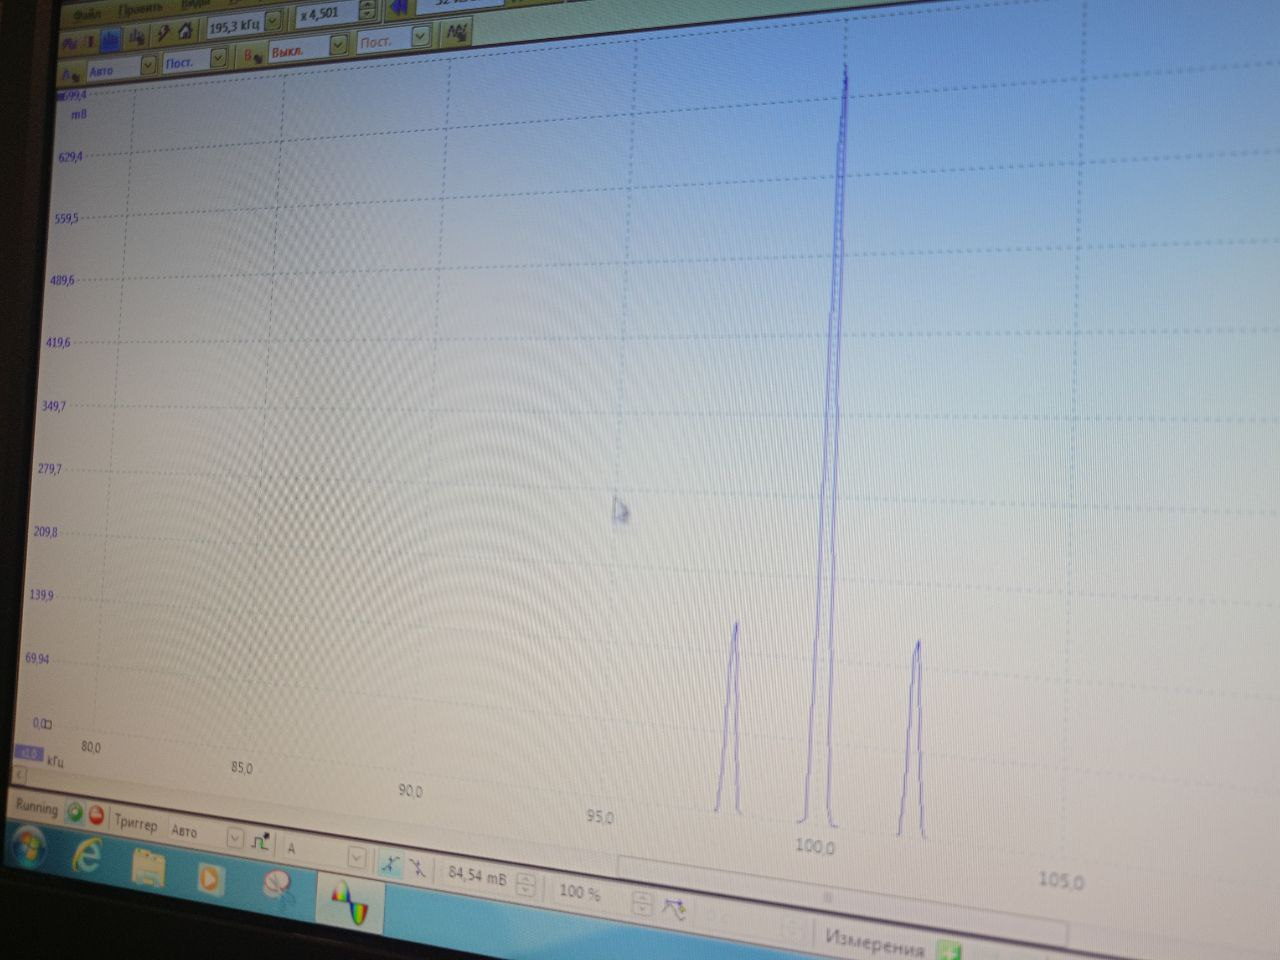
\includegraphics[width=.5\textwidth]{G.21.3.spectr}
    \caption{Сигнал и его спектр при $\nu_{\text{мод}} = 4 \text{кГц}, \nu_0 = 50 \text{кГц}.$}\label{fig:foobar}
\end{center}
\end{figure}

Теперь, изменяя глубину модуляции, запишем в таблицу $a_\text{бок}$ и $a_\text{осн}$ и построим график зависимости $\frac{a_\text{бок}}{a_\text{осн}}(m)$
\begin{figure}[H]
	\begin{center}
    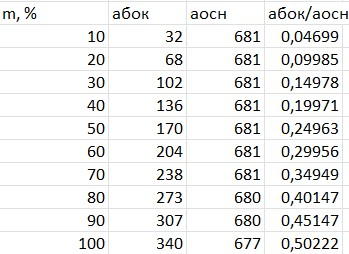
\includegraphics[width=.6\textwidth]{G.23.tabl}
\label{fig:foobar}
	\end{center}
\end{figure}

\begin{figure}[H]
	\begin{center}
    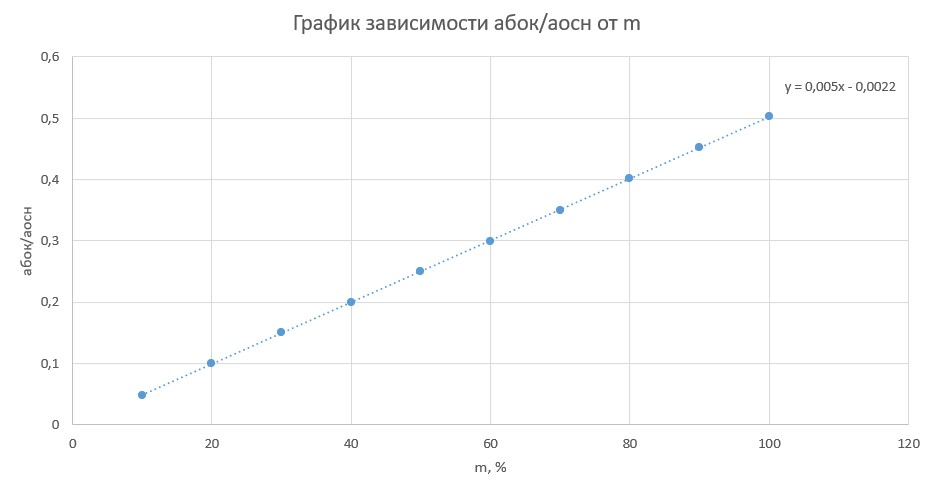
\includegraphics[width=.8\textwidth]{G.23.graph}
\label{fig:foobar}
	\end{center}
\end{figure}

Из графика найдем коэффициент пропорциональности $k = 0,5$, что значит, что $\frac{a_\text{бок}}{a_\text{осн}} = \frac{m}{2}$, что соответствует теории(если взять амплитуды несущего колебания и боковой гармоники, то по формуле получится тот же самый результат).

\subsection*{Изучение фильтрации сигнала}
Для начала возьмем RC цепочку с сопротивлением R = 3 кОм, емкостью конденсатора C = 1000 пФ. Тогда $\tau = 3$ мкс. Подадим последовательность прямоугольных импульсов при различных значениях периода повторения T и рассмотрим форму фильтрованного сигнала и его спектра.

\begin{figure}[H]
\begin{center}
    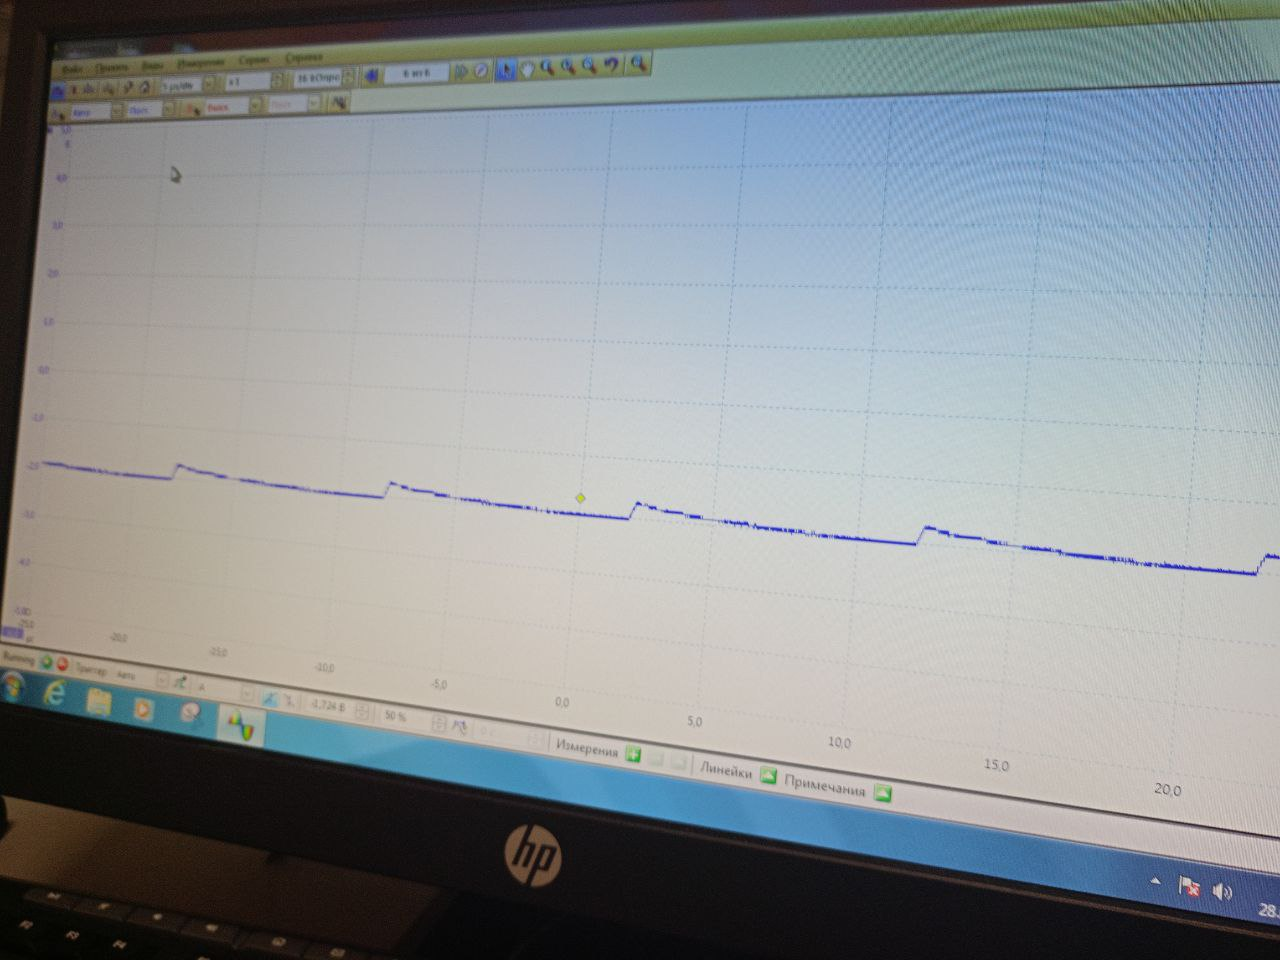
\includegraphics[width=.5\textwidth]{E.30.1.graph}
    \caption{Сигнал при $\tau = 250 \text{нс}, T = 10 \text{мкс}.$}\label{fig:foobar}
\end{center}
\end{figure}

\begin{figure}[H]
    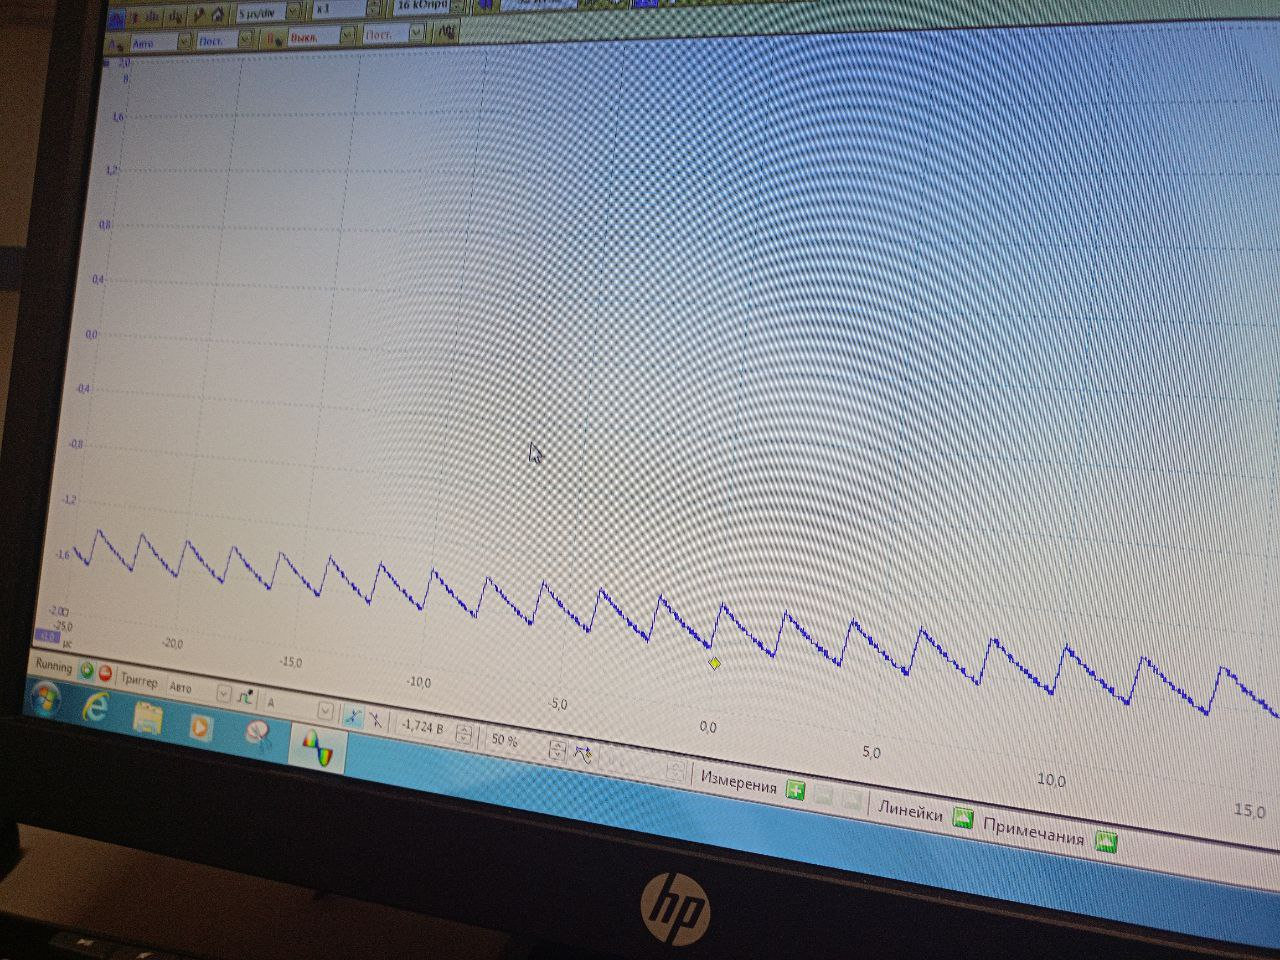
\includegraphics[width=.5\textwidth]{E.30.2.graph}
    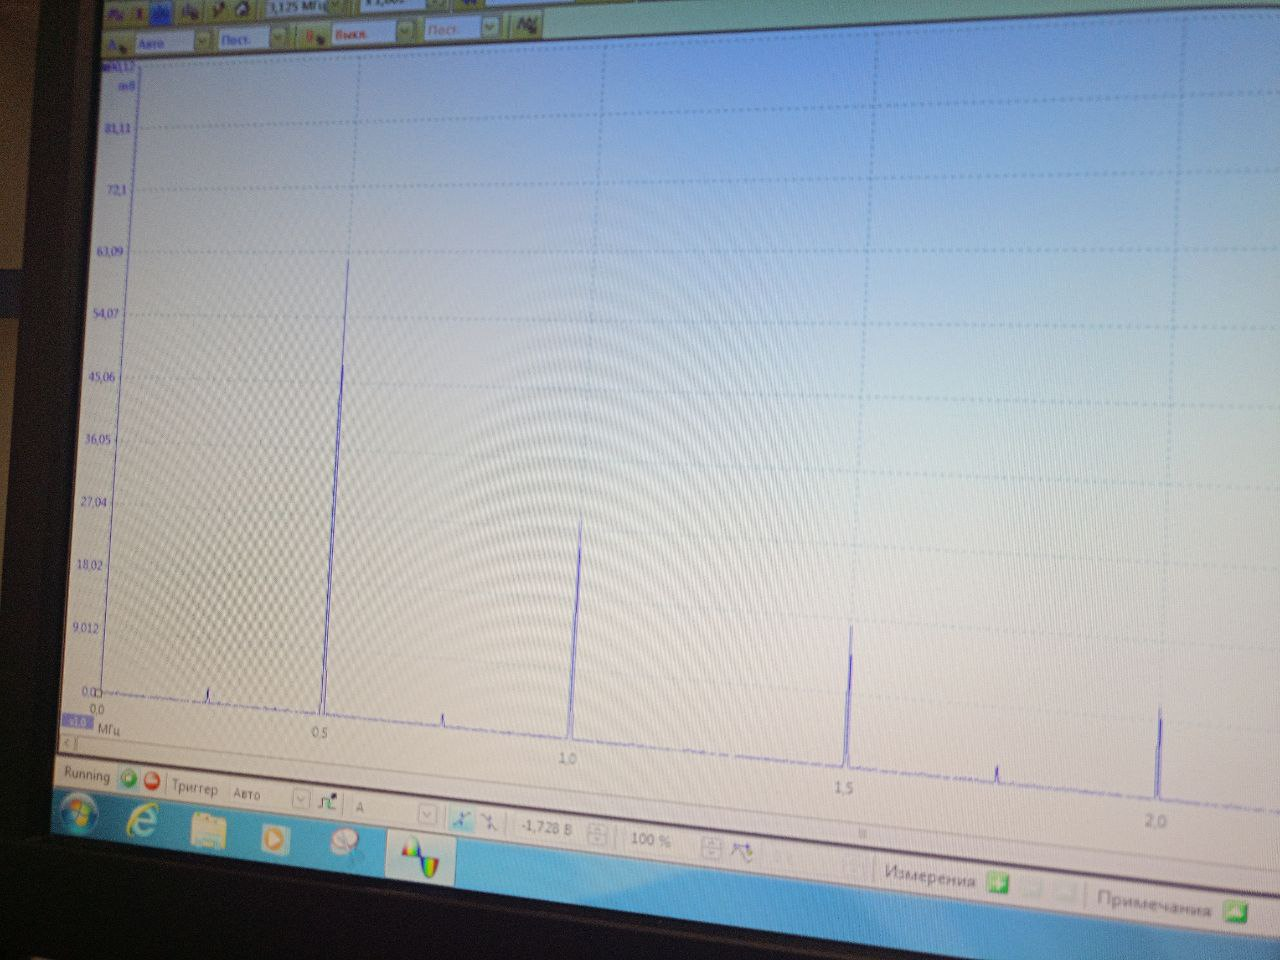
\includegraphics[width=.5\textwidth]{E.30.2.spectr}
    \caption{Сигнал и его спектр при $\tau = 250 \text{нс}, T = 2 \text{мкс}.$}\label{fig:foobar}
\end{figure}

Теперь зафиксируем период T и рассмотрим изменение отношения амплитуд спектральных гармоник при фильтрованном сигнале(подключенном через RC цепь) и исходном сигнале. Данные занесем в таблицу и по ней построим график зависимости $\frac{a_n^\text{Ф}}{a_n}$ от $\nu_n = \nu_0 \cdot n$.

\begin{figure}[H]
	\begin{center}
    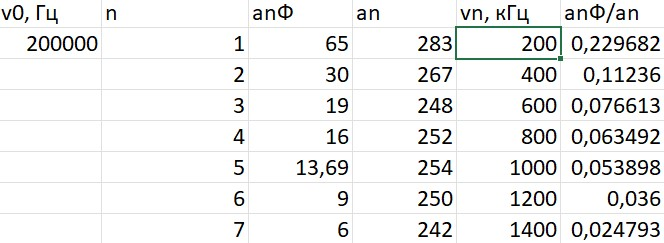
\includegraphics[width=.6\textwidth]{E.33.tabl}
\label{fig:foobar}
	\end{center}
\end{figure}

\begin{figure}[H]
	\begin{center}
    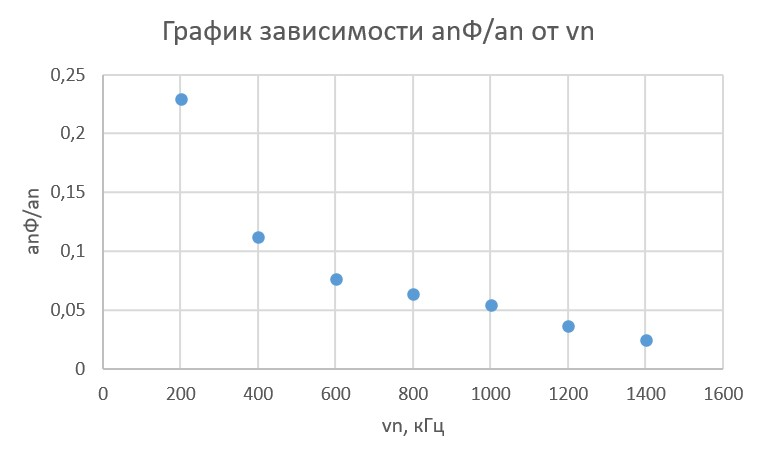
\includegraphics[width=.8\textwidth]{E.33.graph}
\label{fig:foobar}
	\end{center}
\end{figure}

График напоминает гиперболу, что совпадает с теоретическими данными, т.к. характеристическая функция RC цепи имеет гиперболическую зависимость.

\section*{Вывод}
В ходе данной работы были рассмотрены преобразования Фурье, изучены понятия спектра и спектрального анализа, также был исследован спектральный состав периодических электрических сигналов.

Мы изучили прямоугольные импульсы, цуги синусоидальных колебаний, амплитудно-модулированные сигналы, а также филтрованные сигналы. Неоднократно экспериментальным путем было проверено и подтверждено соотношение неопределенности.
\end{document}
